\documentclass{article}
\usepackage{graphicx} % Required for inserting images
\usepackage[hidelinks]{hyperref}
\urlstyle{sf}
\usepackage[nottoc]{tocbibind}  
\usepackage{verbatim} %Package per i commenti
\usepackage[left=2.8cm,right=2.8cm,top=2cm,bottom=2cm]{geometry}
\usepackage{subcaption,graphicx}
\usepackage[none]{hyphenat} 
\usepackage[utf8]{inputenc}  
\usepackage[T1]{fontenc}     
\usepackage{lmodern}         
\usepackage{microtype}      
\usepackage{biblatex}        




\begin{document}
\sloppy


\begin{titlepage}
    \centering

    \vspace*{1cm}
    
    
\includegraphics[width=6cm]{Images/Theory/Logo_UNIPV.svg.png} 
    
    \vspace{1cm}
    
    \textbf{\Large UNIVERSITY OF PAVIA} \\
    \textbf{FACULTY OF ENGINEERING} \\
    \textbf{DEPARTMENT OF INDUSTRIAL ENGINEERING AND INFORMATION}
    
    \vspace{2cm}
    
    \textbf{\Large MASTER’S DEGREE IN COMPUTER ENGINEERING}
    
    \vspace{1.5cm}
    
    {\LARGE \textbf{MASTER THESIS}}
    
    \vspace{2cm}
  
    {\Huge \textbf{Gaze-Based Biometric Authentication Through Dynamic Text Reading}\\[0.8cm]}
    \vfill
    
    
    \begin{flushleft}
        \textbf{Candidate:} Davide Mascheroni \\
        \textbf{Supervisor:} Prof. Marco Porta \\
        \textbf{Co-supervisor:} Piercarlo Dondi and Hoàng Nam Lê \\
        \textbf{Academic Year:} 2024/2025
    \end{flushleft}
    
\end{titlepage}

\newpage
\renewcommand{\contentsname}{Table of contents}
\tableofcontents
\newpage

\begin{abstract}
\setlength{\parindent}{0pt}
\setlength{\parskip}{0.7\baselineskip}
\noindent


\end{abstract}
\newpage

\section{Introduction}
\setlength{\parindent}{0pt}
\setlength{\parskip}{0.7\baselineskip}

\newpage

\section{Behavioural Biometric}
\noindent
In recent years, new information technologies have become increasingly widespread in everyday life. Initially, the most prominent example was the personal computer, but today there is a wide variety of devices available on the market. Currently, the most notable example is the mobile phone. According to Statista [1], in 2024 more than 7.2 billion people worldwide own a smartphone.

All of this has required significant efforts to secure these devices, as they would otherwise be highly vulnerable to attacks.
There exists several layer of security on these devices, but the thesis will mainly focus on a method for verifying a user based on behavioral biometrics.

\subsection{Identification vs Verification}

An important thing to mention is surely the difference between identification and verification.
In fact, this difference represents the basis through which various biometric technologies have been developed.

Identification is the process by which a subject is identified, based on some characteristics that it possesses, from a large number of other subjects.
Identification establishes a user's identity based on the information they provide. This can include a username, email address, or any other information that uniquely identifies them.

Verification is the process by which a machine can verify the correct identity of a subject.
In particular a user can only be accepted or rejected, but not recognized over a large number of users.
Verification confirms that the user is who they claim to be by comparing the information provided by the user against a trusted source, such as a government-issued ID, a passport, or a driver's license.

\subsection{Biometric based on identification}

The most well-known biometric technologies are those based on iris recognition and fingerprint scanning. Unlike traditional passwords, which identify a user through information they know, these technologies rely on intrinsic physical characteristics of the individual. They were specifically developed with the goal of user identification.

Fingerprints are a unique feature that every person has, and can be used to distinguish a person between every other subjects. 
Biometrics uses the fingerprint to identify and authenticate a person.
First, the subject places their finger on a scanner which will be able to save the fingerprint as a biometric profile.
This, unless there are particular accidents in the user's life, will remain the same until death.
After this first step we will move on to the authentication phase.
In this phase the subject will place their finger on the scanner again, which will take the biometric data and compare them with those saved in the previous step.
The outcome of this procedure will be the authentication and identification of a user by the system if the data are matching and a reject if the data differs between them.

Biometric iris recognition uses the intrinsic composition of the human eye to authenticate and identify someone.
The process is similar to that of a fingerprint, with some minor differences in the scanner used to create the biometric profile of a subject.

\begin{figure}[htbp]
    \centering
    \begin{subfigure}[t]{0.45\textwidth}
        \centering
        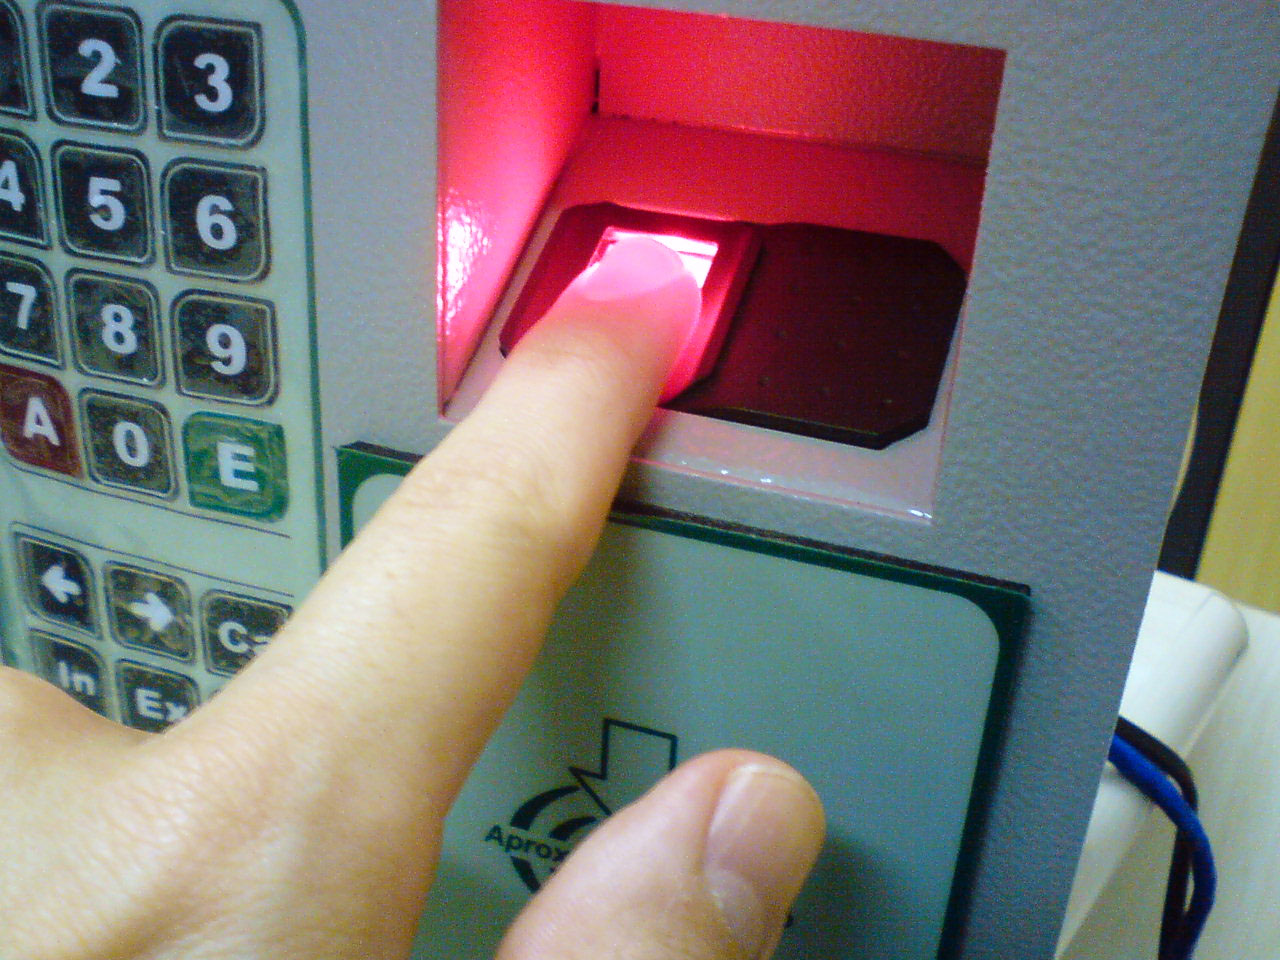
\includegraphics[width=\linewidth]{Images/Theory/Fingerprint_scanner_identification.jpg}
        \caption{Scanner for fingerprint}
        \label{fig:scanner_fingerprint}
    \end{subfigure}
    \hfill
    \begin{subfigure}[t]{0.45\textwidth}
        \centering
        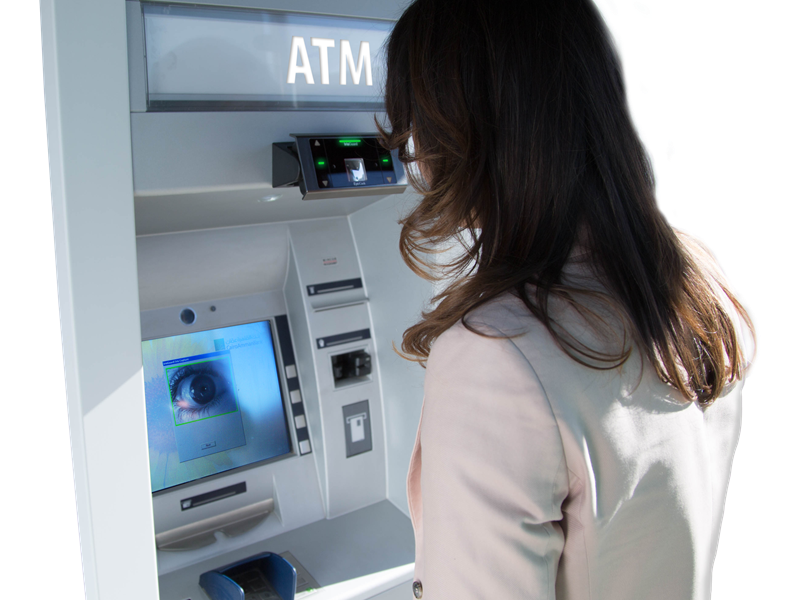
\includegraphics[width=\linewidth]{Images/Theory/eye.png}
        \caption{Scanner for iris recognition}
        \label{fig:scanner_eye}
    \end{subfigure}
    \caption{Different type of scanner}
    \label{fig:scanners}
\end{figure}

The figure \ref{fig:scanners} shows a real world example of scanners used for fingerprint and iris authentication and identification.

As per Nist [2] the best fingerprint systems can reach an accuracy of more than 99\%.
In particular, their test used operational fingerprints from a variety of U.S. and state government sources. A total of 48,105 fingerprint sets from 25,309 individuals, comprising 393,370 distinct fingerprint images, were used in the test.
The performance was based on how many fingerprint images of a person are matched.
The best system was accurate 98.6 percent of the time on single-finger tests, 99.6 percent of the time on two-finger tests, and 99.9 percent of the time for tests involving four or more fingers.
These results were obtained for a false positive rate of 0.01\%, which indicates the people who should have been rejected but were instead accepted by the system.

For what concern the accuracy of iris recognition a Nec [3] study set a benchmark of 99.58\% accuracy.
This study was performed for a 1:N identification problem and it included over 500.000 participants, using both of their eyes for the trial.

As we expected these technology are very strong and reliable because are built over some intrinsic characteristic of a subject.
These characteristics can be used to uniquely identify a person and remain unchanged throughout life.
Another advantage is also that, unlike password-based systems, the user does not have to remember secret information.
Furthermore, it is more difficult to try to authenticate using another person's fingerprint or iris compared to a system based on what a subject knows.

\subsection{Behavioral biometric}

Behavioral biometrics is a discipline primarily focused on the verification problem. Unlike physical biometrics, it does not rely on inherent physical characteristics, but rather on a person’s behavior. Each individual behaves differently, using specific skills or strategies to accomplish tasks in everyday life.
So the machine will be able to collect information about how a subject behave and it will be able to tell us if the user is really who is claiming to be.
As we can expected the behavior is a soft biometric and less robust compared to the fingerprint or iris recognition.
In fact this technology is not used in substitution of the former biometric system, but will be used as another security layer to verify the identity of a subject.
In comparison to the former biometry the system can collect the data in a non intrusive way, without the user even realizing it, and it doesn't need an expensive hardware to do so.

As per Behavioral Biometrics for Human Identification: Intelligent Applications [4] behavioral biometric can be classified in five different categories based on the information about the user being collected:
\begin{itemize}
    \item Authorship based biometric: Is used to collect something that a user produce like a drawing or a written text. Based on this the system will be able to recognize some particular characteristics about the style and verify a subject.
    \item Human Computer Interaction: Every user has a distinctive behavior when interact directly with a machine. The most famous method to do so is certainly the keyboard and the mouse. 
    The way in which the user perform these actions is used as a method for verification.
    \item Indirect HCI-based biometrics: This method is related to the second point, so the interaction of a user with a machine. The goal is to use what the users leaves during the interaction, as an indirect information, to verify it. Some examples of indirect information are audit log, program execution traces and memory usage.
    \item Motor skills: This is probably the best research group because it is based on some characteristic that the user have and learn during his life.
    The motor skill indicate the ability of the user to move muscles in a particular way to perform a task.
    These skills are distinctive to each user and is difficult even to replicate them in the same exact way, so it can be exploited from a verification application.
    \item Purely behavioral biometrics: The last category is based on the pure ability and the behavior used from a user to perform a task. These doesn't measure any muscle movement or something in particular, but it collect all the distinctive action that a user does.
    These actions vary from user to user and are based on the knowledge of a subject or the particular way in which he performs a task.
\end{itemize}

Behavioral biometrics is characterized by several key characteristics. Their universality is limited in the general population because behavioral traits vary in strength or may not exist for everyone. However, when applied in a specific domain, they can achieve full universality since all users are expected to demonstrate the relevant behavior.

In terms of uniqueness, behavioral patterns such as writing styles, gaming strategies, or preferences are not highly distinctive. This makes them more effective for verifying a claimed identity than for identifying individuals in large groups, unless the user base is very small.

Permanence is also a challenge since behavior changes over time as people learn new skills or adapt their techniques. This issue, known as concept drift, is addressed in research on intrusion detection, where adaptive systems are designed to accommodate evolving behaviors.

On the positive side, collectability is straightforward: data can be gathered unobtrusively, often without user awareness, and at low cost. Performance, however, tends to be weaker for identification in large databases, though verification accuracy is generally strong for certain behavioral biometrics.

With respect to acceptability, these methods are often well received due to their non-intrusive nature, though privacy and ethical concerns may arise. 

Finally, circumvention is relatively difficult since it requires deep knowledge of another person’s behavior, but once obtained, imitation can be simple. This highlights the importance of securely encrypting behavioral profiles.

\subsection{Some applications of behavioral biometric}

This section is used to present different real world application of behavioral biometric.
These and other applications are described in Chapter 1, Taxonomy of Behavioral Biometrics, of the book Behavioral Biometrics for Human Identification: Intelligent Applications [4], where they are subdivided into the five categories discussed earlier.
In the thesis only three applications per typology will be represented to have a general overview. Is important to notice that some applications can be characterized with more than one class.

Starting from Authorship based biometric we have a biometric based on sketch recognition. With this method, proposed by (Al-Zubi, Brömme, \& Tönnies, 2003 [5]) , a user is invited to draw a simple sketch of a simple figure, for example some circles, and he can do it freely in the way he wants.
This method captures the distinctive drawing style of the subject, allowing the system to build a model for authentication, achieving an Equal Error Rate (EER) of 7.2\%.
Another example of this category is email behavior used to identify anomalies into mail messages proposed by (Stolfo, Hershkop, Wang, Nimeskern, \& Hu, 2003a; Stolfo, et al., 2003b)[6].
In fact the users follow some habits when they write or read an email.
The time in which the subject reads the mails and empty the mail list, the structure of the mail, the structure of the greetings and the recipient address can be used to create a feature vectors and build a model on that.
The application achieved a detection rate of 90.5\% in identifying suspicious messages.
The programming style is also a method used for authorship and was suggested by Spafford et al. [7]. With this method is possible to recognize who is the author of a program and this is useful to prevent malware or virus, with a detection rate of 73\%.
To create a model the indentation, the comment stile, the programming language used, variable names, type editor and so on are used as features.

The second group of models is the Human and computer interaction class and the email behavior described before is also classified under this name.
Another example is the game strategy approach, in which a player model is build based on his characteristic when he plays.
Yampolskiy et al. [8] proposed a system for verification of online poker players based on a behavioral profile which represents a statistical model of player’s strategy.
Some factors to consider include the range of cards a player holds and the level of aggression in their playstyle. 
This method can be used not only for verification, reaching an EER of 7\%, but also to give other players hints about an opponent
Keystroke method is a method that can also be used for identification. The latter check the pattern used and the style a user uses when typing some characters on the keyboard. For example some users are really fasts while others uses only two fingers to type. We need only to type a short word, like a password, to be able to use this for verification while we need a lot more text if we want to take this model into an identification process.
The keystroke approach for verification was proposed by Bergadano et al. [9], achieving a False Acceptance Rate (FAR) of 0.01\% and a False Rejection Rate (FRR) of 4\%.

The main applications of indirect HCI are surely the audit log, GUI interaction and network traffic.
The audit log is a track that the operating system write automatically about a user activity. CPU and I/O usage, file creation and number of usage of a folder are data collected in a non-intrusive manner and it can be used to verify that the person using the PC is the legitimate user with a detection rate of 93\% and a false positive rate of 8\%.
Given the overwhelming amount of information available, using a random sample is a reasonable approach.
Since the high potential of this approach there are a lot of researches in this field and one of them was performed by Denning, 1987 [10].
While GUI interaction, proposed by  Garg et al. (Garg, et al., 2006) [11], collects data about the interaction of a user with a graphic interface. The collected data enables the creation of advanced behavioral profiles of the system’s users. This comprehensive information can provide insights that are not obtainable from commonly analyzed command-line data.
In fact it reaches a detection rate of 96.15\% and a false positive rate of 3.85\%.
Network traffic analysis has grown significantly in recent years due to the large volume of data arriving from outside the organization. The main focus is to analyse various packet attributes in network traffic, including IP protocol types, packet size, server port numbers, source and destination IP prefixes, Time-To-Live values, IP/TCP header lengths and so on. The goal is to build a user profile based on these data and easily detect a deviation from the normal behavior and mark it as suspect.
Due to the importance of this topic, extensive research has been conducted, including the work of Novikov (2005) [12]. The combined studies achieved a detection rate of 96.2\% with a false positive rate of only 0.0393\%.

One common approach of verification based on motor skill quality was proposed by (Westeyn, Pesti,Park, \& Starner, 2005 [13]; Westeyn \& Starner, 2004 [14]) and is based on blinking. During the creation of the model the user listen a song and blink following the rhythm. Different factor are taken in consideration as the moment in which the user blink, the distance between each of them and the time in which the eye remain closed during that action. After the storage of a subject data is possible to being authenticated blinking again with the same stored song with a detection rate of 82.02\%.
Another famous application is the gait verification method proposed by (BenAbdelkader, Cutler, \& Da
vis, 2002 [15]; Kale, et al., 2004 [16]). The profile of a user is built on the way a user walk taking in consideration the length of the steps, the bounce, distance between the two feet and distance between a foot and the head. This characteristic can changed due to some external factor like pregnancy, body weight or injuries. The advantage of this technique is that can be recorder in a non-intrusive manner using a camera and reaching a detection rate of 90\%.
The keystroke approach, described earlier, is another method that falls into both this category and the HCI category.

The last category is purely behavioral and shares with the authorship category the application of sketch verification.
Another important application of this category is car driving style.
People operate vehicles in very different ways—some drive cautiously and slowly, while others are more aggressive, often speeding or tailgating. Consequently, driving behavior can be considered a form of behavioral biometric. Erdogan et al. (2005a [17]; 2005b [18]) and Erzin et al. (2006) [19] demonstrated that by analyzing variables such as accelerator and brake pedal pressure (in kilogram force per square centimeter), vehicle speed (in revolutions per minute), and steering angle (ranging from \(-720\) to +720 degrees), it is possible to achieve effective genuine versus impostor driver authentication with a detection rate of 88.25\%.
The last example of this class is based on credit card usage.
Data mining techniques are widely applied in credit card fraud detection, often by identifying statistical outliers such as unusual transactions, distant locations, or simultaneous card use. Outlier detection methods rely on distance, density, projection, or distribution analysis. 
Brause et al. (1999) [20] developed a rule-based model using symbolic and analog transaction data, showing that analog data alone is insufficient for reliably detecting fraud with a detection rate of 99.995\% and a FRR of 20\%.

\subsection{Soft Biometric}

Behavioral biometrics is considered a soft biometric approach because it is generally weaker and less stable than traditional biometric systems. Unlike traditional biometric applications, such as fingerprint or iris recognition, which are based on physiological traits that remain largely constant throughout a person’s life, behavioral biometrics rely on dynamic patterns of human activity.

Traditional biometric systems, particularly fingerprint and iris recognition, are regarded as highly reliable and relatively strong approaches. They are built upon physical characteristics that an individual permanently possesses, making them highly distinctive and resistant to change. As noted earlier, these two modalities can reach nearly 100\% accuracy in identification tasks, making them capable of reliably authenticating an individual even within large populations.

By contrast, behavioral biometric technologies can sometimes be applied for identification, but they are generally more suitable for verification tasks. Their typically lower accuracy in identification makes them less suitable as standalone replacements for traditional physiological biometrics. This limitation arises from the fact that behavior is inherently variable: the way a person types, writes, speaks, or drives may change depending on mood, fatigue, health, stress, or environmental conditions.

Nevertheless, behavioral biometrics hold a unique advantage. Unlike traditional biometrics, which often require active cooperation (e.g., placing a finger on a scanner or looking into an iris reader), behavioral systems can operate passively. They collect data continuously in the background, often without explicit effort or awareness on the part of the user. This makes them particularly attractive for continuous authentication scenarios, where the system does not rely on a single login event but instead monitors user behavior throughout a session to ensure that the authenticated person remains the one interacting with the system.

Another strength of behavioral biometrics is their potential to complement traditional systems. For instance, combining fingerprint authentication with continuous keystroke analysis or touch dynamics provides a layered defense: even if a fingerprint is compromised, the behavioral system can still flag anomalies. This layered approach enhances both usability and security, reducing the risk of unauthorized access.

Behavioral biometrics also raise important privacy and ethical considerations. Because these systems can function unobtrusively in the background, they may collect user data without the individual’s explicit awareness. While this capability enhances security, it also underscores the need for strict regulation, informed consent, and robust data protection measures to prevent misuse.



\newpage

\section{Eye tracker}

Before describing an eye tracker we have to understand why the point in which a person is looking is so important.
The reason is that when a person looks at something, they focus on a scene in fine detail and direct their attention to that point.
Therefore, if we can detect where a person is looking during an activity, we can infer their path of attention.
We can also know which part of the scene can be labeled as important for a subject.

\subsection{Visual attention}
Humans receive numerous stimuli during any activity, but they cannot process all of them due to limited cognitive capacity.
As a result, they must select a subset of stimuli they find more interesting or important and focus their processing on those.
The psychologist William James gives the definition of visual attention as:“Many filtered into few for perception”.
This section, according to chapter 1: Visual attention [21], will contain the history of the main study about visual attention during the past years.

\subsubsection{Von Helmholtz’s “Where”}
In the late 19th century, Von Helmholtz (1925) emphasized visual attention as a key mechanism of perception. 
He noted that while attention naturally shifts to new stimuli, it can also be consciously directed even toward peripheral objects without moving the eyes. 
However, he mainly linked attention to eye movements toward spatial locations, which serve as evidence of overt visual attention.

\subsubsection{James’ “What”}
In contrast to Von Helmholtz’s spatial (‘where’) view of attention, James (1981) described attention as an internal, covert process concerned with the identity or meaning of stimuli the ‘what.’ 
These perspectives are complementary, reflecting two aspects of visual processing.
The foveal, or ‘what,’ component enables detailed recognition of central objects, while the parafoveal, or ‘where,’ component guides spatial awareness and directs attention toward peripheral stimuli. 
Together, they illustrate how visual attention integrates object identification with orientation in the surrounding environment.
Although this dual view forms the basis for computational models of bottom-up attention, it is inherently simplistic. 
A comprehensive understanding of visual attention must also account for higher-level, voluntary, and cognitive factors that influence how attention is directed.

\subsubsection{Gibson’s “How”}
In the 1940s, Gibson (1941) introduced intention as a third factor in visual attention, emphasizing the role of advance preparation in shaping reactions. 
His view highlighted the interplay between expectation and intention, showing how perception can shift depending on preconceptions—for example, reading ‘sael’ as ‘seal’ or ‘sail.’ This ‘what to do’ aspect underscores the importance of considering perceptual expectations when designing experiments.

\subsubsection{Broadbent’s “Selective Filter”}
In the 1950s, Broadbent (1958) introduced the ‘selective filter’ model of attention, showing through auditory experiments that while information enters in parallel, it is subsequently filtered into limited-capacity sensory channels.

\subsubsection{Deutsch and Deutsch’s “Importance Weightings”}
Deutsch and Deutsch (1963) opposed Broadbent’s selective filter, proposing instead that all sensory input is processed, with importance weightings determining attention.
Treisman (1971) later reconciled both models by introducing an attenuation filter that weakens, rather than blocks, irrelevant signals, followed by ‘dictionary units’ tuned to importance and context the ‘where’ and the ‘what.’ 
However, the unresolved scene integration problem highlighted how, despite selective perception, we can still construct a coherent overall view of complex scenes, a challenge further explored through eye movement studies and Gestalt theories.

\subsubsection{Yarbus and Noton and Stark’s “Scanpaths”}
Early eye movement studies challenged the Gestalt idea of parallel, holistic visual recognition. 
Yarbus (1967) showed that viewers’ gaze followed sequential patterns when answering questions about an image, while Noton and Stark (1971) identified ‘scanpaths', demonstrating that even without specific instructions, observers tend to fixate on informative regions in variable sequences. 
These findings suggest that a coherent visual scene is constructed piecemeal, supporting James’ ‘what’ aspect of attention, where foveal vision selectively processes regions of interest.

\subsubsection{Treisman’s “Glue”}
Posner et al. and Noton and Stark extended the theories of visual attention originally proposed by Von Helmholtz and James, later integrated by Broadbent and Deutsch \& Deutsch. 
Treisman further unified these ideas through the Feature Integration Theory (FIT), which posits that attention acts as the ‘glue’ binding separate features at specific locations to perceive objects as unified wholes. 
FIT relies on a master map indicating feature locations such as color, orientation, size, and depth while eye tracking is often used experimentally to validate the theory.

\subsubsection{Kosslyn’s “Window”}
Kosslyn (1994) proposed a refined model of visual attention, introducing an adjustable ‘attentional window’ that selectively transmits information from the visual buffer, similar to Broadbent’s and Treisman’s filters. 
The model also posits a redundant, stimulus-based attention-shifting subsystem, relevant to mental imagery, which involves forming internal representations resembling actual perception. 
Notably, eye movements during REM sleep may reflect this internal attentional process, though this remains uncertain.

\subsubsection{Bottom-up model}
Visual attention can be conceptualized through two complementary components: the “what”, corresponding to foveal, object-focused processing, and the “where”, associated with parafoveal, spatial guidance.
In a bottom-up model, peripheral vision first detects salient features at low resolution, which then guide eye movements to reposition the fovea on regions of interest for detailed inspection.
This framework provides a powerful foundation for computational models of visual search, yet it remains incomplete because it does not account for higher-level, voluntary, or cognitive influences.
Voluntary attention enables individuals to selectively focus on areas outside their direct foveal gaze, as demonstrated in scanpath studies and practical examples such as astronomers detecting faint stars through peripheral vision. 
However, while eye tracking offers valuable insights into attentional processes, it is limited to capturing overt eye movements. 
It cannot capture covert shifts of attention, in which focus is redirected without accompanying eye movements, which represents an important limitation for observational studies.”

\subsection{The human eye}

The human eye is a highly specialized organ responsible for capturing light from the environment and transforming it into neural signals that the brain interprets as visual perception.
Its structure is finely adapted to focus incoming light, regulate brightness, and detect a wide spectrum of colors and details.
Understanding the anatomy of the eye is crucial to explain how humans perceive the world, particularly the mechanisms of color vision, which rely on the retina and its photoreceptor cells: rods and cones.

\subsubsection{Anatomy of human the eye}

The human eye is approximately spherical, with a diameter of about 24 millimeters. 

\begin{figure}[ht]
    \centering
    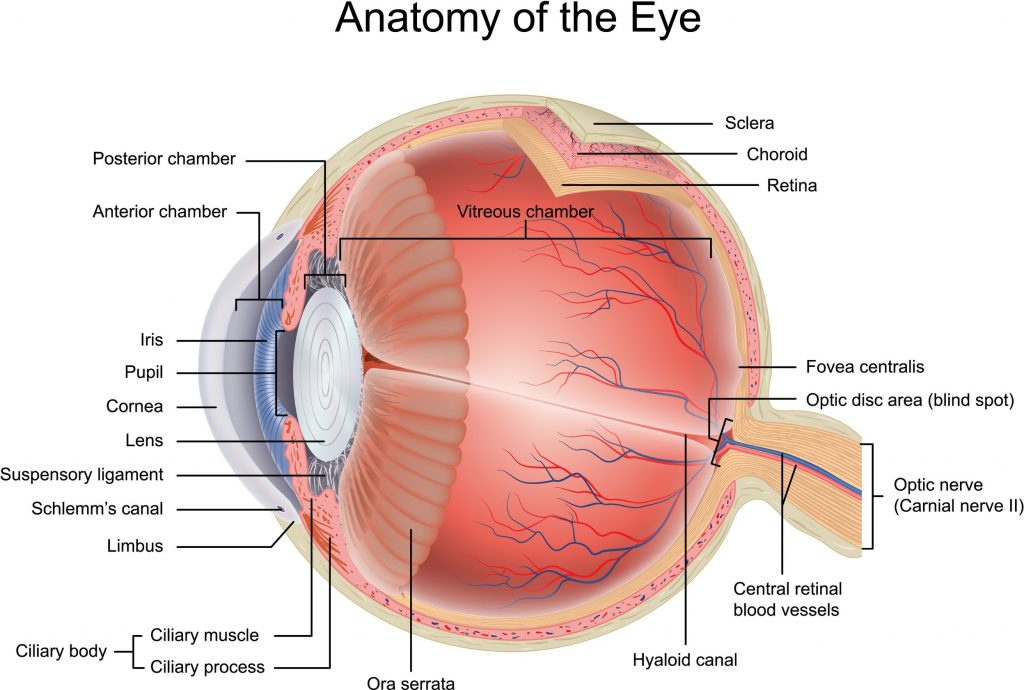
\includegraphics[width = 0.6
    \textwidth]{Images/Theory/occhio.jpg}
    \caption{Anatomy of the human eye}
    \label{fig:ana}
\end{figure}

Despite its relatively small size, it contains an intricate arrangement of structures, each serving a distinct role in the process of vision.
At the very front lies the cornea, a transparent, curved surface that acts as the first point of contact for incoming light. 
Its main function is to bend, or refract, the light so that it can be properly directed toward the deeper structures of the eye.
Just behind the cornea is the iris, the colored part of the eye, which regulates the size of the pupil, the central black opening. 
By widening or narrowing, the iris controls how much light enters the eye, functioning much like the aperture of a camera.
Positioned behind the iris is the lens, a flexible and transparent structure that fine-tunes focus. 
Through the action of tiny ciliary muscles, the lens can change its shape, allowing the eye to adjust focus when shifting between near and distant objects, a process known as accommodation.
Light then travels to the retina, a delicate layer of neural tissue lining the back of the eye. 
Far from being a passive screen, the retina actively processes the incoming light signals. 
It contains specialized photoreceptor cells, rods and cones, that convert light into electrical impulses. 
These signals are then transmitted through the optic nerve, a dense bundle of nerve fibers, to the brain’s visual cortex, where they are interpreted and transformed into meaningful images.

\subsubsection{The retina and photoreceptor}

As we said earlier the retina plays a central role in vision, functioning as the site where light is transformed into neural signals that the brain can interpret. 
Within this thin layer of tissue reside two main types of photoreceptor cells, namely rods and cones, each of which is adapted for specific visual tasks.

\begin{figure}[ht]
    \centering
    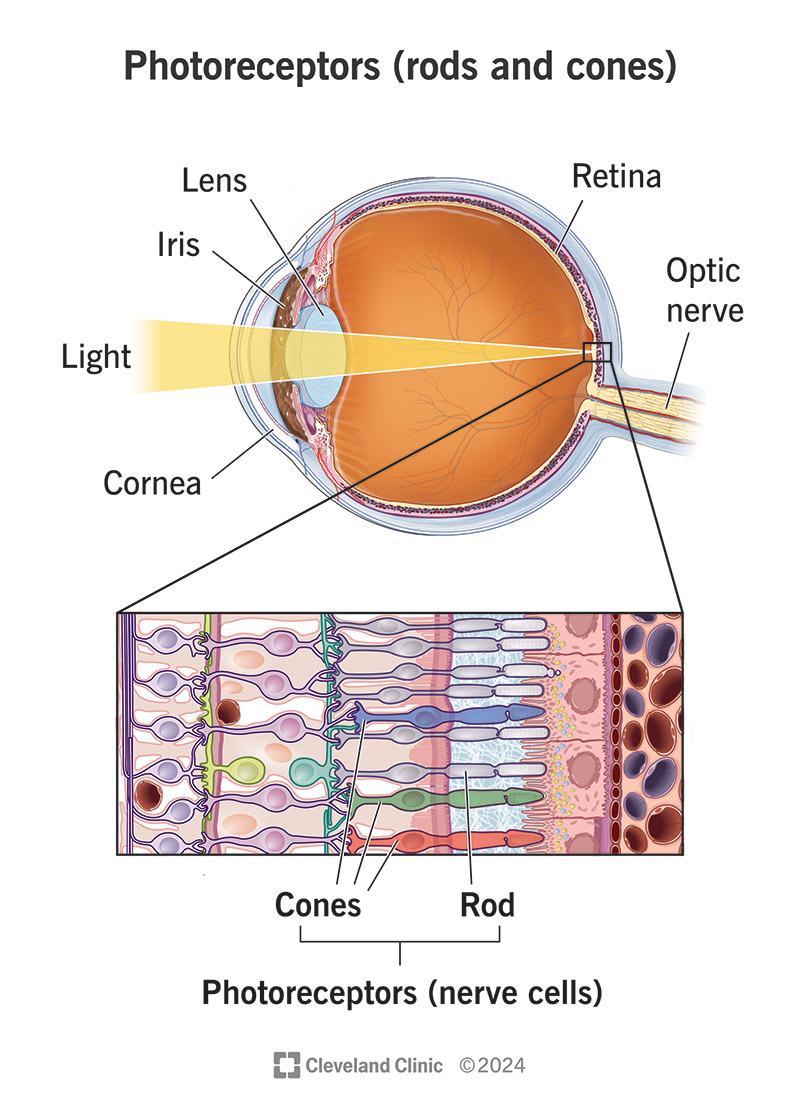
\includegraphics[width = 0.4
    \textwidth]{Images/Theory/rods_cones.jpg}
    \caption{Rods and Cones}
    \label{fig:rodscones}
\end{figure}

Rods are highly sensitive to light and enable vision under low-light conditions. 
Although they do not mediate color perception, they are essential for detecting shapes, movement, and variations in brightness. 
Humans possess approximately 120 million rods in each eye, with the majority concentrated in the peripheral regions of the retina. 
This distribution explains why peripheral vision is far more effective in low-light environments, even though it lacks the ability to discriminate color.
Cones, by contrast, are less sensitive in low-light conditions but are indispensable for perceiving color and fine detail.
About 6 million cones are found in each eye, most of them concentrated in the central retina and especially within the fovea, a small depression that provides the sharpest visual acuity.
Cones are divided into three subtypes according to the wavelengths of light to which they are most responsive.
Some are sensitive to short wavelengths corresponding to blue light, others respond to medium wavelengths associated with green, and still others detect long wavelengths corresponding to red. 
The combined activity of these three types of cones forms the basis of human trichromatic vision, enabling us to perceive the full spectrum of visible colors.
This characteristic explains why the RGB color model is among the most widely used frameworks in digital imaging and display technologies.

\subsubsection{Color perception}

The process of color perception begins when incoming light stimulates the cones. 
Each cone type has a broad response curve, meaning that their sensitivity ranges overlap. 
The brain does not simply interpret the activity of a single cone in isolation, but instead compares the relative responses of the three cone classes to determine the perceived color. 
For instance, strong activation of long-wavelength cones with weaker responses from the other two is interpreted as red. 
When medium- and long-wavelength cones are equally stimulated while short-wavelength cones contribute little, the result is perceived as yellow. 
If all three types respond at similar levels, the visual system interprets the signal as white. 
Thus, color vision is not a direct reading of individual wavelengths but an emergent property of neural comparison and integration across multiple cone pathways.
The interaction between rods and cones further illustrates the complexity of human vision.
Cones dominate during daylight conditions, but as light diminishes, rods become increasingly important.
This shift, known as the Purkinje effect, reflects the higher sensitivity of rods to blue-green wavelengths.
As a result, red objects appear to darken as twilight falls, while blue ones remain more easily visible. 
Such changes highlight the complementary nature of rods and cones: one system optimized for detail and color in bright environments, and the other specialized for sensitivity in low-light conditions.

\subsubsection{Type of eye movements}

Human vision is not a static process. 
The eyes are in constant motion, guided by a sophisticated neuromuscular system that allows the fovea, the central region of the retina responsible for high acuity, to be directed toward relevant visual targets.
These movements are not random, but are precisely coordinated to stabilize images, explore the environment, and ensure that critical details are perceived accurately.
Almost all normal primate eye movements can be classified into five basic types: saccadic, smooth pursuit, vergence, vestibular, and physiological nystagmus.
Each serves a distinct function, yet together they form an integrated system that balances accuracy, stability, and adaptability in visual perception.

Saccades are rapid, ballistic shifts of the eye that redirect the fovea from one point of interest to another.
They are the fastest of all eye movements, reaching velocities of up to 900 degrees per second, and typically last only a few tens of milliseconds. 
Despite their speed, saccades are precisely controlled, allowing humans to scan text when reading, explore complex scenes, or quickly detect changes in the environment. 
During saccades, visual sensitivity is temporarily reduced through saccadic suppression, preventing motion blur and maintaining visual stability.

In contrast to the abruptness of saccades, smooth pursuit movements allow the eyes to follow a moving object with remarkable fluidity. 
These movements are slower, generally limited to about 100 degrees per second, but are highly adaptive to the velocity of the target.
Smooth pursuit depends on both visual feedback and predictive mechanisms, as the eyes often anticipate the trajectory of an object to maintain accurate tracking.
This function is particularly critical for activities such as driving, sports, or any task where continuous monitoring of moving stimuli is required.

Vergence refers to the inward or outward rotation of the eyes that aligns them with targets at different depths.
Unlike saccades or pursuit, vergence movements are disjunctive: the two eyes move in opposite directions.
Convergence occurs when the eyes rotate inward to focus on a near object, while divergence refers to outward rotation for distant viewing. 
These adjustments are essential for depth perception and binocular vision, allowing humans to perceive the world in three dimensions.
Vergence movements are slower than saccades but are tightly linked with accommodation of the lens to maintain clear and unified images across distances.

The vestibular system, located in the inner ear, interacts with eye movements to ensure visual stability during head motion. 
The vestibulo-ocular reflex (VOR) automatically generates compensatory eye movements that counteract head displacement, allowing the gaze to remain fixed on a target even when the body is in motion.
For example, when walking or turning the head, the VOR maintains stable vision by producing equal and opposite eye rotations. 
This reflex is exceptionally fast, with response latencies of just a few milliseconds, underscoring its role in stabilizing vision in dynamic environments.

Although the eyes may appear still when fixating on an object, they are never completely motionless.
Physiological nystagmus refers to small, involuntary movements—including tremors, drifts, and microsaccades—that occur during fixation. 
These tiny displacements prevent the image on the retina from fading due to neural adaptation. 
Without them, stationary objects would gradually disappear from perception. Physiological nystagmus, therefore, is a crucial mechanism for maintaining continuous visual awareness of the environment, even when the gaze is held steady.

Though described separately, these five types of movements rarely operate in isolation. 
In natural vision, they combine seamlessly to provide both stability and flexibility.
For instance, during visual search, saccades bring the fovea to regions of interest, smooth pursuit maintains focus on moving targets, vergence adjusts for depth, vestibular reflexes stabilize the gaze against body motion, and physiological nystagmus ensures constant retinal stimulation.
Together, they form a dynamic and adaptive system that underpins the human ability to explore, interact with, and interpret the visual world.

\subsubsection{Fixation}

Fixation is the process by which the eyes maintain their gaze on a single point, allowing the visual system to capture and process detailed information from the environment.
Although the eyes may appear motionless during fixation, they are in fact never completely still.
Tiny involuntary movements such as microsaccades, tremors, and drifts occur constantly, preventing the image on the retina from fading due to neural adaptation and ensuring continuous visual awareness. 
These subtle motions are essential for maintaining clarity and precision, as they allow the fovea, the central region of the retina responsible for high-acuity vision, to remain accurately aligned with the target.
Fixation is fundamental to how humans interact with the visual world.
It provides a stable platform for extracting fine details, enabling activities that require careful attention, such as reading, inspecting objects, or monitoring a complex scene.
During fixation, the visual system is able to prioritize relevant information, enhancing perception and supporting higher-level cognitive processes such as attention, memory, and decision-making.
Even in dynamic environments, fixation works in concert with other eye movements: after rapid saccades redirect the fovea to a new location, fixation allows the visual system to stabilize and analyze the target.
While during smooth pursuit of moving objects, brief fixations may occur to refine the image and maintain accuracy.
Physiological nystagmus during fixation further ensures that retinal stimulation is continuous, allowing the perception of stationary objects to remain vivid and precise.
In essence, fixation is not merely a passive pause of the eyes but a dynamic and intricate process.
It balances stability and subtle motion, integrating seamlessly with other eye movements to support accurate, continuous, and detailed visual perception.
Without fixation, the human ability to explore, interpret, and respond to the environment with precision would be significantly impaired, highlighting its critical role in the visual system

\subsection{Eye tracking techniques}

After recognizing the importance of eye movements, it becomes clear that we need a tool to track them, and this tool is called an eye tracker.
In the past, eye trackers were highly expensive devices, mostly limited to research labs and specialized industries.
Over the years, however, their price has steadily decreased, making the technology more accessible.
Today, affordable solutions are available not only for scientific research but also for commercial applications such as gaming, marketing, user experience studies, and even healthcare.
This reduction in cost has opened the door to new innovations, allowing eye tracking to move from a niche tool to a widely adopted solution across many fields.
Eye trackers can be divided into two main categories: those that measure the position of the eye relative to the head and those that measure the orientation of the eye in space, also known as the Point of Regard (POR).
Building on this distinction, Chapter 5 of Eye Tracking Methodology: Theory and Practice [21] further identifies four methodological approaches to eye movement measurement: Electro-Oculography (EOG), scleral contact lens or search coil methods, Photo-Oculography (POG) or Video-Oculography (VOG), and video-based techniques combining pupil and corneal reflection.

\subsubsection{Electro-OculoGraphy (EOG)}

Electro-oculography (EOG) was the predominant method for recording eye movements around forty years ago and, although less common today, it still finds use in both clinical and research settings.
The technique operates by detecting differences in the corneo-retinal standing potential, which are measured through electrodes placed on the skin surrounding the eye. The recorded signal typically falls within the range of 15 to 200 µV, with a nominal sensitivity of approximately 20 µV per degree of eye movement. While EOG is effective for capturing eye movements relative to head position, it lacks the precision required for determining the point of regard. Consequently, its application for gaze tracking is limited unless combined with complementary systems capable of monitoring head movements, such as head trackers.

\subsubsection{Scleral Contact Lens/Search Coil}

One of the most accurate ways to measure eye movements uses a mechanical or optical reference attached to a contact lens that is worn directly on the eye. 
Early versions of this method, dating back to the late 19th century and later developed by Young and Sheena (1975) [22], used a plaster-of-Paris ring placed on the cornea, connected by mechanical linkages to recording devices.
Modern implementations use a scleral contact lens, which covers both the cornea and part of the sclera (the white of the eye) to prevent the lens from slipping.
A small mounting stalk is attached to the lens, and various devices can be placed on this stalk, such as reflective markers, line diagrams, or wire coils.
In magneto-optical eye-tracking systems, the wire coil is the most commonly used device. The coil is attached to the contact lens and moves together with the eye. 
As it rotates within a carefully controlled electromagnetic field, the system detects changes in the coil’s orientation and generates precise measurements of eye movement. This setup allows extremely fine tracking of even very small rotations of the eye, making it one of the most accurate methods for recording eye position.
Based on Young and Sheena researches [22] the scleral search coil is extremely precise, with an accuracy of about 5–10 arc-seconds over a small range of roughly 5°. 
However, it is also highly invasive. 
Inserting the lens requires practice and care, and wearing it can be uncomfortable. 
In addition, this method measures the eye’s position relative to the head, so it is generally not suitable for directly determining the point of regard.

\subsubsection{Photo-OculoGraphy (POG) or Video-OculoGraphy (VOG)}

This category includes a wide range of eye movement recording techniques that rely on measuring distinct features of the eye during rotation or translation. 
Examples include the apparent shape of the pupil, the position of the limbus (the boundary between the iris and the sclera), and reflections from a nearby directed light source, often in the infrared spectrum. 
Although the specific methods differ, they are grouped together because they generally do not provide direct measurements of the point of regard. 
Measurements of ocular features in these techniques may be obtained either automatically or manually.
Manual visual inspection, such as reviewing recorded eye movements frame by frame on videotape, is extremely time-consuming, prone to error, and limited by the temporal sampling rate of the video device.
Automatic limbus tracking typically uses photodiodes mounted on spectacle frames and generally relies on invisible illumination, usually in the infrared range. Many of these methods also require the head to be held still, commonly using a head or chin rest, or a bite bar, to reduce movement (Young and Sheena, 1975)[22].

\subsubsection{Video-Based Combined Pupil/Corneal Reflection}

While the previously discussed techniques are generally suitable for measuring eye movements, they often do not directly provide point-of-regard measurements.
To determine the point of regard, either the head must be stabilized so that eye position relative to the head corresponds to gaze direction, or multiple ocular features must be tracked to distinguish between head movements and eye rotations.
Two key features commonly used for this purpose are the corneal reflection of an infrared light source and the center of the pupil.
Video-based eye trackers employ relatively inexpensive cameras and image-processing systems to calculate the point of regard in real time. 
These systems may be table-mounted or head-mounted.
The optical principles behind both configurations are essentially the same, with size and portability being the main differences.
Modern video-based eye trackers are compact and often integrated into monitors, making them particularly suitable for interactive applications.
In these systems, the corneal reflection, also known as a Purkinje image, is measured relative to the pupil center.
The human eye generates four distinct Purkinje reflections, which are formed by light reflecting off different surfaces within the eye: the anterior and posterior surfaces of the cornea, and the anterior and posterior surfaces of the lens (Crane, 1994) [23].
Each reflection carries unique optical information, but most video-based eye tracking systems rely primarily on the first Purkinje reflection, which is produced by the anterior corneal surface. 
This reflection is the brightest and most stable, making it well suited as a reference point for calculating gaze direction when measured relative to the pupil center.
With proper calibration, these trackers can reliably map a viewer’s point of regard on a planar surface where calibration targets are displayed. 
Tracking both the pupil center and the corneal reflection allows the system to separate eye rotations from minor head movements.
Specifically, the relative position between the pupil and the first Purkinje reflection changes with eye rotation but remains nearly constant with small translations of the head.
More advanced systems, known as generation-V eye trackers, also measure the fourth Purkinje reflection (Crane \& Steele, 1985) [24].
These dual-Purkinje image (DPI) eye trackers can distinguish between translational and rotational eye movements: both reflections shift equally during translation, but they move differently during rotation, allowing the separation of the two effects.
Although highly accurate, DPI systems often still require the head to be stabilized for optimal performance. 
This is because even small head translations or rotations can introduce noise into the measurement, making it difficult to distinguish subtle eye movements from head motion. Stabilization methods, such as chin rests, bite bars, or other mechanical supports, are therefore commonly used to minimize artifacts.
While this limitation reduces the comfort and naturalness of the setup, it ensures the precision needed for research applications that demand extremely fine measurements of gaze direction.

\begin{figure}[ht]
    \centering
    % First row
    \begin{subfigure}[b]{0.45\textwidth}
        \centering
        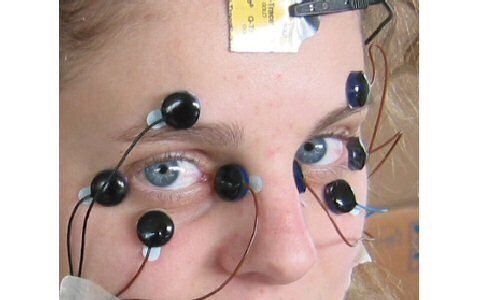
\includegraphics[width=1\textwidth,height=0.6\textwidth]{Images/Theory/eog.png}
        \caption{Electro-OculoGraphy (EOG)}
        \label{fig:eog}
    \end{subfigure}
    \hfill
    \begin{subfigure}[b]{0.45\textwidth}
        \centering
        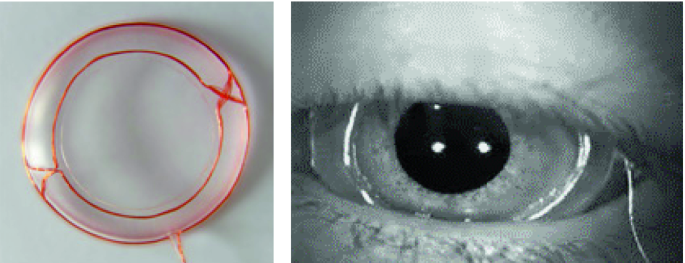
\includegraphics[width=1\textwidth,height=0.6\textwidth]{Images/Theory/coil.png}
        \caption{Scleral Contact Lens/Search Coil}
        \label{fig:coil}
    \end{subfigure}
    
    \vspace{0.5em}
    
    % Second row
    \begin{subfigure}[b]{0.45\textwidth}
        \centering
        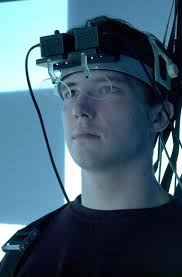
\includegraphics[width=0.7\textwidth,height=0.6\textwidth]{Images/Theory/vog.jpeg}
        \caption{Video-OculoGraphy (VOG)}
        \label{fig:vog}
    \end{subfigure}
    \hfill
    \begin{subfigure}[b]{0.45\textwidth}
        \centering
        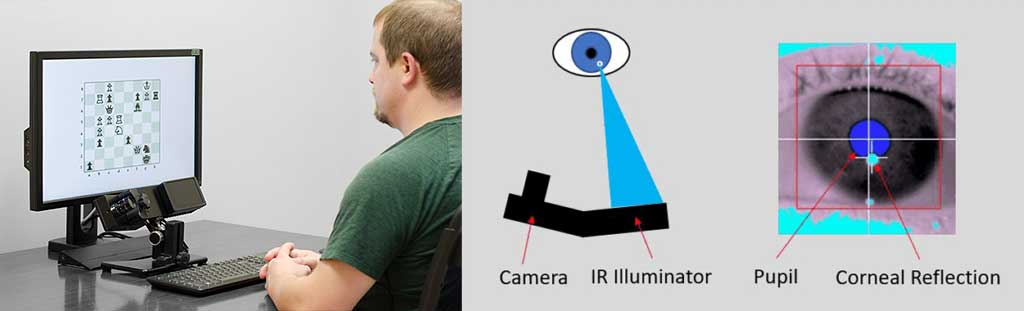
\includegraphics[width=1\textwidth,height=0.6\textwidth]{Images/Theory/corneal.jpg}
        \caption{Corneal Reflection}
        \label{fig:corneal}
    \end{subfigure}

    \caption{Different types of eye tracker}
    \label{fig:four_grid}
\end{figure}

\newpage
\section{State of the art}

This section presents an updated overview of the state of the art in gaze-based biometric solutions.
As a starting point, we draw on the work presented in Chapter 9 – Biometric Authentication to Access Controlled Areas Through Eye Tracking [25], published in 2017. Building upon this foundation, the review is expanded to include significant experimental studies and technological developments that have emerged in the years since, with particular attention to contributions up to 2025.
In this chapter, we deliberately exclude methods that rely on static characteristics of the human eye, such as iris-based recognition, which are already well established in biometric research. 
Instead, we focus on dynamic approaches, in which identity-related information is derived either from the manner in which an individual visually interacts with stimuli or from temporal changes in particular ocular characteristics.
The way an individual explores a visual scene, whether in a free-viewing context or under controlled conditions, can reveal distinctive patterns that serve as biometric cues.
In addition, time-dependent changes in ocular features, such as variations in pupil diameter, may provide further information useful for identity verification or recognition.
Building on this perspective, five principal categories of eye-tracking-based biometric techniques will be considered. 
The first includes ATM-like solutions, which simulate practical authentication scenarios.
The second focuses on fixation and scanpath analysis, where the sequence and duration of gaze points are examined. 
The third category emphasizes eye and gaze velocity, capturing the dynamics of eye movement. 
The fourth examines pupil size variations, which may be influenced by both physiological and cognitive factors.
Finally, the fifth category explores oculomotor characteristics and head orientation, integrating motor control features of the visual system into biometric assessment.

\subsection{ATM-LIKE SOLUTIONS}

This section begins with a review of gaze-driven authentication systems, which have been developed as alternatives to traditional password or PIN entry methods.
Such systems are particularly relevant in contexts resembling Automated Teller Machines (ATMs), where secure and efficient user authentication is essential. 
By replacing manual input on a keyboard with gaze-based interactions, these approaches aim not only to improve usability but also to reduce vulnerabilities such as shoulder surfing or keylogging, while at the same time opening new possibilities for integrating behavioral traits into the authentication process.
While these solutions are not strictly biometric, since the underlying information often comes from sequences of alphanumeric characters or graphical symbols, the way such sequences are entered through eye movements introduces behavioral elements that may carry biometric value.
For this reason, these approaches merit discussion as precursors to fully gaze-based biometric methods.

One of the earliest contributions in this area was presented by Maeder et al. [26], who explored gaze-directed authentication based on consciously fixating predefined regions of a visual stimulus for specified durations.
In their study, participants were shown an image of Prague divided into a non-uniform 3 × 3 grid.
Each user selected six “points of interest,” with one in each grid cell, and authentication was achieved by reproducing the same sequence of fixations.
In this design, the gaze path effectively served as a PIN, while the grid structure ensured both consistency and flexibility.

A further step toward practical implementations was proposed by Kumar et al. [27] in their system EyePassword, which aimed to reduce vulnerabilities such as shoulder surfing and eavesdropping. 
Four input modalities were compared: a traditional keyboard, gaze plus manual confirmation on an on-screen QWERTY keyboard, gaze with dwell time on a QWERTY layout, and gaze with dwell time on an alphabetic layout.
Although average entry times across the dwell and trigger-based methods were comparable (between 9.2 and 12.1 seconds), error rates were notably higher when a manual trigger was used (15\% versus 3–4\%).
These results highlighted both the feasibility of gaze input for secure authentication and the trade-offs between speed, accuracy, and usability.

In another line of research, De Luca et al. [28] proposed the use of eye gestures as authentication tokens. 
This method was inspired by the observation that visual patterns or geometric shapes are often easier to memorize than long alphanumeric strings. 
Here, authentication was performed by “drawing” gestures on the screen with the gaze, using eight basic directional strokes originating from or directed toward the screen’s center. 
Such gestures represented an alternative form of input, combining memorability with the natural motor control of the eyes.

Similarly, Dunphy et al. [29] replaced numeric or textual credentials with a recognition-based scheme relying on faces. 
Users were asked to memorize a set of faces during an initial training phase and later authenticate by selecting them from sequences of grids containing distractor images. This approach emphasized recognition rather than recall, exploiting the human visual system’s efficiency in face perception.

Other researchers explored the use of gaze interaction with symbolic keyboards. 
Weaver et al. [30] developed a system where authentication was achieved by looking at symbols arranged on a virtual keyboard.
Instead of relying solely on dwell time for character selection, gaze points were clustered and automatically analyzed to infer the intended input, thereby reducing delays and improving fluidity.

More recently, Cymek et al. [31] investigated authentication through smooth pursuit eye movements, which occur when the gaze follows a continuously moving target.
Their method used a moving PIN pad where each digit followed a unique trajectory, defined by a sequence of up, down, left, or right movements.
Authentication was achieved by tracking the trajectory of the correct digits with the eyes. 
Although this technique was slower than traditional dwell-time input, it offered distinct advantages: it reduced the need for calibration and made it more difficult for attackers to infer the entered PIN, since the input was encoded in movement patterns rather than in static gaze points.

Khamis et al. [37] conducted a rigorous comparison of cue-based authentication modalities for situated displays, focusing on touch, mid-air gestures, and calibration-free gaze. 
Through two in-depth user studies (N = 20, N = 17), they highlighted a clear tradeoff between usability and security. 
Gaze input was found to be more secure against shoulder-surfing attacks, but it was also more demanding and slower.
Mid-air gestures offered slightly higher security than touch, though they were less favored in public contexts.
Touch, on the other hand, remained the fastest but was less secure.
Their findings underline important design implications for balancing efficiency, security, and user acceptance in public authentication scenarios.

Omair Shahzad Bhatti et al. [36] proposed a calibration-free authentication method for interactive public displays based on saccadic eye movements, addressing the limitations of slower gaze-based approaches. 
In a user study with ten participants, their method was compared against CueAuth, a smooth pursuit-based system by Khamis et al. [37]. The results showed a substantial improvement in accuracy (82.94\% to 95.88\%) and a significant reduction in entry time (from 18.28s to 5.12s), making the approach comparable to touch-based input in speed while maintaining strong security.

Authentication systems are now widely used to protect personal information, but common approaches such as PINs, biometrics, and smart cards remain vulnerable. 
PINs are easily exposed through shoulder-surfing, biometrics can be spoofed, and smart cards are at risk of theft or duplication. 
To address these limitations, ADIL HAMID MALLA [38] proposes a gaze-based authentication system designed to counter shoulder-surfing, video-based observation, and spoofing attempts.
Experimental results demonstrate the effectiveness of the approach, achieving an accuracy of 97.5\% (F-measure = 0.97) in authenticating legitimate users and 89.5\% (F-measure = 0.89) in detecting intruder attempts.

Eye tracking has gained attention as a promising tool for biometric authentication, as eye movements are fast, distinctive, and require minimal effort from users.
However, earlier gaze-based systems often struggled with high error rates or slow authentication.
To address these issues, Ivo Sluganovic et al.[39] developed a method that uses reflexively triggered eye movements through interactive visual stimuli, enabling reliable feature extraction within seconds and eliminating the need for memorization. 
An additional advantage is that the stimulus can be uniquely generated for each login attempt, supporting a challenge–response mechanism that defends against replay attacks. 
A prototype tested with 30 participants demonstrated strong performance, achieving an equal error rate of 6.3\% and reducing authentication time to about 5 seconds, outperforming many prior approaches.

Matin Fallahi et al. [40] proposed a multimodal biometric authentication system for Extended Reality (XR), addressing the usability and security limitations of password-based methods. 
Traditional password entry in XR is cumbersome and error-prone, often leading to weaker password choices and reduced security. 
To overcome this, their approach combines eye movement patterns with brainwave signals, using consumer-grade sensors that can be seamlessly integrated into XR devices.
A prototype tested with 30 participants achieved an exceptionally low Equal Error Rate (EER) of 0.29\%, significantly outperforming single-modality systems based on eye movements (1.82\%) or brainwaves (4.92\%), as well as state-of-the-art biometric methods (EERs between 2.5\% and 7\%).
Importantly, this solution supports seamless and immersive authentication through visual stimuli, eliminating the need for complex user interactions.

Traditional authentication methods such as passwords overlook personal behavioral traits of users.
This study, suggested by Cantoni et al. [44], explores the use of eye-tracking data for biometric purposes during PIN entry via an on-screen virtual numeric keypad.
Both identification and verification are investigated. 
Machine learning algorithms are applied to analyze gaze patterns across the full PIN sequence as well as at the level of individual digits. 
The results, while not achieving the precision of traditional biometrics, are satisfactory within the context of soft biometrics, where the goal is to complement existing authentication methods—here, the PIN itself—by providing an additional layer of security.

Haochen Wang [47], in his thesis, presents four case studies evaluating gaze-based biometrics, including doorbell name inspection for building access, static image observation, moving target observation, and eye-driven soft PIN input.
Both identification and authentication were tested, including an analysis of user familiarity in the building access study. 
Results showed classification accuracies above 0.7 across most experiments, demonstrating the feasibility of gaze-based biometrics as a viable “soft biometric” method when combined with traditional authentication techniques.

\subsection{METHODS BASED ON FIXATION AND SCANPATH ANALYSIS}

The use of fixations and scanpaths for biometric applications has been investigated for over a decade.
One of the earliest contributions was by Silver and Biggs [53], who compared keystroke dynamics with eye-tracking data for identification purposes. 
Although keystroke-based models clearly outperformed gaze-based ones, this work was among the first to highlight the potential of eye tracking as an alternative technique for biometric verification.

Subsequent studies have sought to extract and refine gaze features for improved performance. 
Holland and Komogortsev [54], for example, examined reading scanpaths using a high-frequency eye tracker (1000 Hz) and a dataset of 32 participants. 
They employed a wide range of features, such as fixation count, average fixation duration, and saccade amplitudes, as well as aggregate scanpath descriptors including path length, area, and inflection count.
By applying Gaussian cumulative distribution similarity measures and feature fusion, they achieved their best result with an Equal Error Rate (EER) of 27\%. 

In later work, Holland and Komogortsev [55] expanded this line of inquiry using both high-end (1000 Hz) and low-cost (75 Hz) eye trackers. 
From 32 and 173 participants, respectively, they extracted fixation and saccade features, which were analyzed with several statistical tests and machine learning classifiers. 
Their approach produced an EER of 16.5\% and a rank-1 identification rate of 82.6\%, demonstrating the potential of combining traditional statistics with machine learning for gaze-based biometrics.

Alternative methodologies have also been explored. 
Rigas et al. [56] introduced a graph-based approach in which fixations on face images were clustered using a minimum spanning tree (MST) technique.
Comparing overlap in MST structures between subjects enabled user identification with accuracies ranging from 67.5\% to 70.2\% across 15 participants and eight sessions.

Galdi et al. [57] conducted an experiment involving 88 participants across three sessions. 
Sixteen grayscale facial images were used as stimuli, and each image was divided into 17 Areas of Interest (AOIs) corresponding to facial regions (e.g., eyes, mouth, nose). 
For each participant, feature vectors were constructed by calculating the average fixation duration per AOI across all images. 
Using Euclidean and Cosine distance measures for comparison, the system achieved its best performance with combined features, reaching an Equal Error Rate (EER) of 0.361.

Cantoni et al. [33] extended this approach with a larger participant pool (111 from the first study plus 24 additional subjects one year later) and introduced the Gaze ANalysis Technique (GANT). 
Instead of manually defined AOIs, an automatic face normalization algorithm was applied to divide each image into a uniform 7×6 grid (42 cells).
Weights were calculated for each cell based on fixation density and duration, as well as for arcs connecting cells to capture gaze transitions. 
Similarity between models was assessed by comparing difference matrices via the Frobenius norm. Trials with both single and combined features showed that the best results were achieved when all features (density, fixation duration, and weighted paths) were fused, yielding a minimum EER of 28\%.

Further contributions expanded the scope of gaze-based biometrics beyond identity verification. Cantoni et al. [58] and Galdi et al. [59] applied features derived from GANT datasets to gender and age classification.
Using Adaboost and Support Vector Machines, they reported moderate success, with gender classification rates near 60\% and age classification rates around 55\%.

Other research has focused on task dynamics as a differentiating factor. Biedert et al. [60], for instance, examined task learning effects to detect unauthorized system access. 
They hypothesized that genuine users would navigate familiar interfaces fluidly, while impostors would exhibit higher exploratory behavior. 
To quantify this, they introduced the Relative Conditional Gaze Entropy (RCGE) method, which analyzes gaze distribution patterns.

Finally, George and Routray [61], winners of the BioEye 2015 competition, developed a highly effective approach to biometric identification. 
Using recordings from 153 participants across three sessions (two separated by 30 minutes and one by one year), they extracted extensive fixation and saccade features and applied backward feature selection with a Radial Basis Function Network (RBFN). 
Their method achieved success rates of 98\% across the shorter interval and 94\% across the one-year interval, highlighting the robustness of gaze-based biometrics under temporal variability.

Yin et al. (2022) [34] proposed a gaze-based authentication method leveraging the spatiotemporal features of eye movements.
To address the long recording times required by previous approaches, their method uses shorter eye movement recordings, recommending durations under 12 seconds based on deviations between gaze points and stimuli.
Temporal motion of gaze points and spatial saccade patterns were used to represent individual identity.
Experiments on two datasets (5 s and 12 s recordings) showed that open-set Equal Error Rates (EER) reached 10.62\% for 12 s and 12.48\% for 5 s, while closed-set EERs were 5.25\% and 7.82\%, respectively, demonstrating the method’s effectiveness for rapid, eye-movement-based authentication.

The COVID-19 pandemic underscored the need for contactless authentication methods, particularly those based on eye or gaze features, which remain effective even when users wear masks and can complement traditional password or PIN systems. 
In this context, Porta et al. [35] presented a study on gaze-based soft biometrics that employed simple animations as visual stimuli, in which small squares moved along different patterns and trajectories without the need for preliminary calibration of the eye tracker. 
Machine learning analysis of the collected data demonstrated strong performance, especially in verification tasks, achieving accuracies above 80\% and Equal Error Rates (EER) often below 10\%.

The study, suggested by Yasmeen Abdrabou et al. [48], explores using gaze behaviour to assess perceived password strength, aiming to help users select passwords resistant to guessing attacks. 
We propose incorporating users’ understanding of password strength into security mechanisms by analysing gaze patterns during password creation.
In a proof-of-concept study (N = 15), participants created both weak and strong passwords.
Results show that password strength can be predicted from gaze behaviour with 86\% accuracy using machine learning, paving the way for novel interfaces that encourage stronger password choices.

B. L. Tait [83] proposed a study in which 25 participants employed the EyeWriter eye-tracking system to assess whether individual eye movement behavior is sufficiently distinctive for secure biometric authentication.
The results indicate that behavioral eye movements can be effectively employed for biometric verification, particularly in a one-to-one authentication context, achieving success rates between 96\% and 100\%.
In contrast, one-to-many identification yielded an accuracy of only 21.83\%. 
While this demonstrates some potential, the limited sample size restricts the generalizability of the findings and highlights the need for further investigation with larger populations.

With the emergence of Virtual Reality (VR) displays equipped with embedded eye trackers, eye-tracking data is increasingly accessible and can be leveraged for applications such as gaze monitoring, privacy protection, and user authentication.
User identification is particularly critical in VR due to security and privacy concerns. 
Previous work has primarily relied on machine learning applied to motion-based data (e.g., body, head, eye, and hand tracking), typically requiring explicit tasks and extensive feature sets. 
In contrast, Asish SM et al. [84] proposed a system for user identification based on minimal eye-gaze features, without the need for identification-specific tasks. 
To evaluate user identification, gaze data from an educational VR application were processed with machine learning models (RF, kNN) and deep learning models (CNN, LSTM).
Results demonstrate that all models achieved identification accuracies exceeding 98\% using only six simple gaze features. 
The findings underscore the potential of eye-gaze–based identification in VR, while emphasizing its security and privacy implications and acknowledging the limitations of the current study.

\subsection{METHODS BASED ON EYE/GAZE VELOCITY}

Bednarik et al. [62] investigated the potential of eye velocity as a distinguishing feature for biometric purposes.
They considered left-eye, right-eye, and combined velocity signals.
However, the results indicated very limited discriminative power, with identification rates ranging only between 6\% and 25\%.

Kinnunen et al. [63] proposed an approach based on the distribution of gaze angles over short temporal windows. 
The local velocity direction of the eyes was estimated using trigonometric transformations and represented in normalized histograms. 
Seventeen participants watched a 25-minute video while gaze data were collected at 120 Hz. 
Each participant was modeled using Gaussian Mixture Models, following a methodology reminiscent of speaker recognition. 
Depending on the amount of training and testing data available, error rates varied between 29.4\% and 47.1\%, reflecting moderate performance.

Rigas et al. [64] examined velocity and acceleration as biometric indicators by applying the Wald–Wolfowitz statistical test to compare distributions of dynamic eye features.
Their experimental design used a moving dot as stimulus, which jumped every 550 ms within grids of either 3×3 (Dataset A) or 2×2 (Dataset B) positions. 
Data were collected from 37 and 79 participants respectively, yielding 978 and 4168 signals. 
Fixations were extracted from these signals, and the classification results were encouraging, with identification rates of 96.6\% for Dataset A and 90.4\% for Dataset B.

Cuong et al. [65] introduced an alternative representation by encoding gaze features with Mel-Frequency Cepstral Coefficients (MFCCs). 
Features such as eye position, eye difference, and velocity were transformed into MFCC representations and classified using a single multi-class classifier, where the stimulus was represented by a moving point.
This approach emphasized the potential of signal-processing methods borrowed from speech recognition for eye-movement biometrics.

Liang et al. [66] explored acceleration-based features, focusing particularly on diagonal movements and one and two step shifts in both horizontal and vertical directions.
Five participants were instructed to repeatedly watch short video clips, and their eye movements were analyzed using both Back-Propagation neural networks and Support Vector Machine classifiers. 
The highest accuracy achieved in their work reached 82\%, suggesting that acceleration properties can provide stable biometric signatures even with relatively small sample sizes.

Darwish and Pasquier [67] concentrated on saccadic dynamics as a biometric source. 
Their study recruited 22 participants, with eye movements recorded at 120 Hz across four sessions scheduled twice weekly.
Stimuli included various patterns, such as a 4×4 dot matrix.
From the eye-movement data, several features were derived, including angular velocity and acceleration (for both left and right eyes) as well as absolute velocity. 
Mean, standard deviation, and maximum values of these metrics were then computed and used to train a Random Forest classifier with 10-fold cross-validation. 
This approach achieved strong results, with a Half Total Error Rate (HTER) of around 5\%.

Holland and Komogortsev [68] also incorporated velocity-based features into their framework.
Specifically, they extracted horizontal and vertical mean velocity along with peak velocities in both directions.
These parameters were used as part of a larger feature set to test classification models across datasets collected with both high-frequency and low-cost trackers.

Yoon et al. [69, 70] proposed a classification framework using velocity categories modeled through Hidden Markov Models (HMMs). 
In their first study [69], eye movements were captured from 12 participants with a 60 Hz eye tracker while they observed 250 still images composed of structured dot patterns (proximity grids, aligned grids, glass patterns, large shapes, and small shapes).
Velocity data were grouped into five states: extremely low velocity, fixation, smooth pursuit, saccade, and extremely high velocity. 
Using HMMs with five hidden states, classification accuracies ranged from 53\% to 76\%, with higher performance observed for participants with lower average gaze velocity. 
The second study [70] extended the analysis to 16 participants tested over morning and afternoon sessions. 
Here, HMMs were individualized by selecting the best likelihood across 2–5 hidden states per user.
While classification accuracies decreased to between 17\% and 41\%, the results confirmed that lower gaze velocity correlated with higher accuracy. 
They also noted better results for morning sessions, suggesting that fatigue might impair biometric consistency.

Juhola et al. [71] and Zhang et al. [72] focused on saccadic features for verification tasks. Juhola et al. compared data acquired from two eye trackers with very different sampling rates (400 Hz vs. 30 Hz) while participants followed a dot moving along a black bar.
They extracted amplitude, accuracy, latency, and maximum velocity of saccades and tested Linear Discriminant Analysis, Quadratic Discriminant Analysis, and Naive Bayes classifiers. 
High-frequency data led to recognition rates of around 90\%, whereas low-frequency recordings yielded 70–90\%. 
Zhang et al. extended this line of work by analyzing longer-term stability, with test intervals ranging from half a day to 16 months, using a 30 Hz tracker.
They added maximum acceleration and deceleration as features and employed classifiers such as Learning Vector Quantization, Discriminant Analysis, Naive Bayes, and Support Vector Machines. 
Verification experiments achieved up to 86\% accuracy for genuine users and 88\% for impostors with SVMs.

Srivastava et al. [73] combined velocity features with position and difference based features in an SVM multi-class classification framework. 
Using a moving point stimulus, their model consistently achieved high accuracy, exceeding 91\% across different test scenarios.

Finally, Eberz et al. [74] also incorporated temporal descriptors of saccadic dynamics into their biometric framework, focusing particularly on speed and acceleration.
These features were analyzed in conjunction with pupil size, thereby integrating both movement-based and physiological signals.
By combining dynamic saccade characteristics with pupillary responses, their study aimed to capture a richer representation of user-specific visual behavior. 
This multimodal approach demonstrated that temporal aspects of saccades, when fused with pupil-based metrics, can enhance the distinctiveness of biometric profiles and contribute to more reliable user identification.

Ali, Hoque, and Deravi [45] proposed a presentation attack detection method based on directed gaze trajectories, where randomized visual stimuli are used to trigger natural pupillary motion, making spoofing attempts harder to succeed. 
Their system was tested with photo, 2D mask, and 3D mask artifacts on data collected from 80 volunteers.
The results demonstrated that gaze trajectory features are effective in distinguishing genuine users from presentation attacks, confirming the potential of this approach for enhancing biometric security in practical applications.

Spoofing is a major challenge for biometric systems, and a gaze-based method using randomized visual stimuli has been proposed to detect such attacks.
Ali et al. [46] propose a method based on the idea that natural head–eye coordination during gaze shifts creates unique accuracy patterns that are difficult for impostors to mimic.
Data collected from genuine users and from attackers employing photographs, 2D masks, or replayed videos were analyzed using features derived from collinear and colocated gaze points. 
Experimental results, including both isolated feature evaluations and score-fusion combinations, demonstrated the effectiveness of the method in distinguishing between authentic and spoofed attempts.

Harezlak K et al. [49] evaluated biometric identification using eye movement signals by testing new features, including frequency-domain representations and the largest Lyapunov exponent, alongside velocities and accelerations.
Eye movement data were recorded in 100-ms segments from 24 participants across two sessions, as they observed a point appearing at 29 screen locations. 
Feature vectors were created for single points and sequences of three points. 
Two training/testing scenarios were tested: one with 75\% of randomly selected vectors and equal participant representation, and another using separate sessions for training and testing.
Decision tree and random forest classifiers performed best, with random forest achieving up to 100\% accuracy in the first scenario, while performance dropped significantly in the second.

\subsection{METHODS BASED ON PUPIL SIZE}

Despite receiving relatively limited attention as a biometric trait, pupil size has emerged as a promising indicator for both identification and verification, as evidenced by several noteworthy investigations.

Bednarik et al. [62], previously discussed in relation to other ocular features, also examined the role of pupil size in biometric recognition. 
Their experimental setup included 12 participants exposed to four types of visual stimuli: text, a static cross, a moving cross, and an image.
The features extracted comprised pupil size (left, right, and combined), delta pupil size (for left, right, and combined), eye velocity (left, right, and combined), and interocular distance.
In addition, aggregate mean values of these attributes were examined, and the analysis employed Fast Fourier Transform (FFT), Principal Component Analysis (PCA), as well as their combined application.
Performance was assessed using both individual features and weighted feature fusion. 
The best single-feature result was achieved with eye distance, yielding a 90\% success rate.
However, as this measure relates more closely to physical rather than behavioral characteristics, its biometric validity is limited.
Among behavior-related features, delta pupil size achieved the strongest outcome (60\%). When feature fusion was applied, combining eye distance with other features consistently resulted in accuracies exceeding 90\%.

Nugrahaningsih and Porta [75] extended this line of inquiry by evaluating pupil size as a soft biometric in a longitudinal setting. 
Their study involved 25 participants tested across two sessions separated by one year. 
The experimental task was minimal, requiring subjects only to fixate on a plus sign displayed at the center of a white background.
Key attributes included left and right pupil sizes, along with their ratio and difference.
Each attribute was described by 15 statistical measures (e.g., minimum, maximum, mean, variance, median, geometric mean, harmonic mean, interquartile range, kurtosis, skewness, and range). 
Additional features included the sum of squared differences and the correlation between left and right pupil sizes.
Classification was performed using four algorithms: Naïve Bayes, Neural Networks, Support Vector Machines (SVM), and Random Forests.
Results indicated higher identification performance when selected subsets of features were employed (0.6194–0.7187), while verification performance remained consistently strong across both full and reduced feature sets ( $\approx$0.97).

Eberz et al. [76] further explored the discriminative power of pupil size by incorporating it into a larger framework of 21 features.
Pupil-based measures included maximum, minimum, mean, standard deviation, and range of pupil diameter. 
Participants were instructed to click as quickly as possible on red dots with white centers that appeared sequentially in random screen locations.
Three experimental conditions were used: no prior instruction, textual guidance, and a visual preview of the dot locations. 
In addition to pupil features, temporal and spatial eye-movement features were also considered. 
Classification was performed using k-Nearest Neighbors (kNN) and Support Vector Machines. 
Across the three experimental settings, equal error rates (EER) ranged from 3.98\% to 9.27\%, underscoring the value of combining pupil size with dynamic ocular features for reliable biometric identification.

The following work, proposed by Casanova et al. [51], develops a web user identification model by analyzing behavioural biometrics from touch dynamics and periocular characteristics such as pupil movements, blinks, and fixations.
A feature-level fusion approach is applied, combining different distance measures (Euclidean, Bray-Curtis, Manhattan, Canberra, Chebyshev, Cosine) to determine whether a test sample matches the target subject.
Multi-data processing methods such as Canonical Correlation Analysis (CCA) and Principal Component Analysis (PCA) are used to further enhance performance.
Results show that fusing these biometric traits significantly improves accuracy, achieving over 92\%, surpassing individual biometrics.

\subsection{METHODS BASED ON OCULOMOTOR FEATURES}

Kasprowski and Ober [77] investigated the use of Cepstral analysis, the inverse Fourier transform of the logarithm of a signal’s power spectrum, as a biometric feature.
Eye movement data were collected with a 250 Hz tracker from nine participants instructed to follow a 3×3 jumping point stimulus, with each participant enrolled on 30 occasions. 
The dataset consisted of “probes” representing eye movement recordings during eight-second stimulations. 
From these data, 15 cepstral coefficients were extracted across four waveforms and subsequently used as input to four classifiers: K-Nearest Neighbors (KNN), Naïve Bayes, Decision Tree, and Support Vector Machine (SVM). 
Classification performance was assessed using 10-fold cross-validation, yielding an average False Accept Rate (FAR) of 1.48\% and a False Reject Rate (FRR) ranging between 6.7\% and 43.3\%, with an overall average of 22.59\%.

Building on different physiological properties, Komogortsev et al. [78] examined oculomotor plant characteristics (OPC) as a verification biometric. 
Their method extracted saccadic parameters from eye-tracking data and transformed them into nine OPC components using a linear homeomorphic 2D oculomotor plant model. 
These components included length tension, series elasticity, passive viscosity, agonist and antagonist force–velocity relationships, tension intercept, agonist and antagonist tension slopes, and eye globe inertia. 
Two statistical techniques—Student’s t-test with Voting and Hotelling’s T² test—were employed to measure similarity between OPC vectors, with an additional AND/OR fusion strategy to combine classifier outcomes. 
Using a 1000 Hz eye tracker, data were collected from 59 participants across two sessions separated by a 20-minute break, during which participants followed a jumping dot stimulus. 
The best result achieved was a minimum Half Total Error Rate (HTER) of 19 \%, using both Hotelling’s T² test and the OR Student’s t-test with Voting for horizontal saccadic data.

In a subsequent contribution, Komogortsev et al. [79] explored a multimodal ocular biometric framework by integrating three distinct traits: OPC, Complex Eye Movement (CEM) patterns, and the physical structure of the iris.
While iris recognition is not the primary focus of this survey, it was included in their study alongside OPC and CEM features, both derived from eye movement dynamics captured via image sequences. 
A Sony PlayStation Eye camera was employed to record both iris and eye movement data, using Rorschach inkblot images as stimuli.
Data from 87 participants were analyzed, and results demonstrated that combining these ocular traits improved overall accuracy and enhanced the resistance of the system against spoofing attempts.

Finally, Liang et al. [80] complemented their use of acceleration-based features by integrating muscle properties into the framework, with particular attention to seven “optimum muscle parameters.”
These parameters were derived to capture the biomechanical characteristics of the oculomotor system, reflecting how individual differences in muscular control influence eye movement dynamics.
By integrating these physiological descriptors into their biometric model, the authors demonstrated that muscle-based features can provide complementary information to traditional kinematic measures, thereby enhancing the distinctiveness and reliability of gaze-driven biometric identification.

Dillon Lohr et al. [42] investigated the fusion of two eye-centric authentication modalities—eye movements and periocular images—within a calibration-free framework. 
While both modalities have demonstrated promise individually, their integration in a unified pipeline had not been studied extensively at scale.
Using a large in-house dataset of 9,202 subjects with eye-tracking quality comparable to consumer-grade VR devices, the authors showed that their multimodal approach consistently outperformed unimodal systems and surpassed the FIDO benchmark.
The use of advanced machine learning models enabled the system to capture complementary discriminative features from both modalities, significantly enhancing authentication performance.

In 2023 Alessandro D’Amelio et al. [43] proposed a principled framework for modeling eye movements as a form of behavioral biometrics, drawing on foraging theory as a basis for capturing the uniqueness of individual gaze behavior. 
A composite Ornstein–Uhlenbeck process is employed to characterize the exploration–exploitation dynamics of eye movements, with parameters inferred from eye-tracking data through Bayesian analysis.
These parameters serve as discriminative features for biometric identification, which is performed using standard classification techniques.
A proof of concept on a publicly available dataset demonstrates the effectiveness of the approach, highlighting its potential both for biometric applications and for advancing the analysis of eye-tracking data.

The increasing need for secure digital access, coupled with technological advances and the lack of standardized solutions, continues to drive research into eye movement–based biometrics.
This work, suggested by Harezlak and Plucienni[81], presents two neural network–based approaches to user identification from eye movement dynamics.
In the first method, a 100-element time series was constructed to represent eye movement features, including velocity, acceleration, jerk, point-to-point percentage changes, and frequency-domain characteristics. 
These were modeled using a Long Short-Term Memory (LSTM) network. 
The second method employed the same dynamic features but derived statistical descriptors from the time series, which were then classified using a dense neural network.
Experiments were conducted with the publicly available GazeBase dataset, focusing on recordings obtained under the “jumping point” stimulus condition. 
Results demonstrate strong discriminative potential: the LSTM model with time series feature vectors achieved 96\% accuracy, while the statistical feature–based method achieved 76\%. 
These outcomes were observed across a three-year span of recordings, with analyses also considering different temporal segments and stimulus configurations.

The work suggested by Abbas Seha et al. [85] examines the biometric potential of eye movement patterns from low frame rate eye-tracking devices.
It also explores recognition improvements through additional static and dynamic ocular features, such as eye blinking patterns and periocular shape characteristics.These modalities are relevant for applications like continuous driver authentication in law enforcement. 
Two datasets were collected using different low frame rate eye trackers, recording eye movements from 55 participants during real driving sessions. 
For eye gaze, fixation and saccade features—including duration, amplitude, and statistical descriptors—were extracted.
Blinking features included patterns, speed, acceleration, and power-per-unit-mass profiles, while periocular features comprised eye-opening height, width, and axial ratio. 
Each modality was evaluated individually, then combined in a multi-modal fusion. While single modalities showed moderate performance, fusion of static and dynamic features significantly improved results, achieving up to a 98.5\% recognition rate and 0\% error rate. 
This demonstrates that, although single-modality approaches may lack robustness, multi-modal fusion offers high reliability for continuous driver authentication.

\subsection{METHODS BASED ON HEAD ORIENTATION}

Cazzato et al. [32] introduced an alternative to traditional eye trackers by employing the depth and RGB streams of the Microsoft Kinect sensor.
Their approach did not aim to precisely determine the exact gaze point.
Instead, it relied on cases where head orientation could be treated as a reasonable approximation of gaze direction, followed by a rough estimation of pupil position.
Because gaze could not be assessed in every video frame due to computational delays and occasional failures in detecting the face or pupil, the missing values were estimated using Kalman Filter predictions. 
The gaze detection process consisted of two stages. In the first stage, head pose was estimated using the depth and RGB data. 
In the second stage, pupil position was determined from the RGB stream. 
These two components were then combined to calculate the final X and Y gaze coordinates. 
Feature extraction was carried out using Principal Component Analysis (PCA), and the selected features were classified through a Minimax classifier.
Experiments were conducted with 12 participants who watched three short video clips. 
The results showed that precision ranged from 81\% to 83\%, while recall ranged from 80\% to 86\%.

M. Wierzbowski et al. [50] conducted an investigation involving 43 participants who viewed multiple 360-degree VR videos while their eye-tracking data and headset orientation were recorded.
Using both deep learning and classical statistical methods, the researchers tested whether a viewer of a previously unseen VR video could be identified based on prior viewing data. 
The experiments achieved a maximum average identification accuracy of 75\%, demonstrating the potential for identifying VR users under unforced behavioural conditions.

This research, conducted by Rubo et al. [52], investigates the feasibility of implicit user identification in Social Virtual Reality (VR) based solely on eye gaze patterns during dyadic interactions.
Employing Siamese Convolutional Neural Networks on data from 128 participants, the study achieved an identification accuracy of 95.50\% by combining models for gaze during speaking and listening. 
Findings indicate that gaze patterns constitute distinctive, idiosyncratic behavioral traits, largely independent of self-reported personal characteristics.
These results underscore significant privacy and security implications for Social VR environments, where gaze data may be collected passively under conditions of limited movement and variable data quality.

Identifying users of a Virtual Reality (VR) headset enables adaptive interface design, personalization of settings, and adjustment of difficulty levels in both gaming and training applications.
While most existing identification methods require explicit input, implicit user identification offers a less intrusive alternative that preserves immersion.
Liebers et al. [82] proposed a biometric identification system leveraging gaze patterns and head orientation during stimulus tracking for user recognition.
The method was validated through a user study, with a hybrid post-hoc analysis yielding identification accuracies of up to 75\% using an interpretable machine learning model and up to 100\% with a deep learning approach.
Finally, potential application scenarios are discussed, demonstrating how this approach can enable seamless and implicit user identification in VR environments.

Recent research has explored identifying users in virtual reality (VR) based on behavioral data. 
These approaches often rely on elaborate authentication tasks resistant to “shoulder surfing” but overlook whether identification is possible under natural behavior.
In the study by Wierzbowski et al. [86], involving 43 participants, the authors investigated whether a viewer of an unseen 360° VR video could be identified using eye-tracking and headset orientation data recorded while viewing other 360° VR videos.
Using deep learning and classical statistical methods, we achieved up to 75\% average identification accuracy, demonstrating the potential for VR user identification under unforced conditions.


\section{experiment}
\subsection{Preliminary experiments}
\subsection{Feature captured with eye tracker and description of the tool}

\section{Appendice}
\section{Conclusion}
\noindent
\section{Acknowledgment}


\newpage
\section{References}
[1] Number of smartphone mobile network subscriptions worldwide from 2016 to 2023, with forecasts from 2023 to 2028, \url{https://www.statista.com/statistics/330695/number-of-smartphone-users-worldwide/}

[2] NIST study shows computerized fingerprint matching is highly accurate, \url{https://www.nist.gov/news-events/news/2004/07/nist-study-shows-computerized-fingerprint-matching-highly-accurate}

[3] NIST study shows computerized fingerprint matching is highly accurate, \url{https://www.nec.com/en/press/202109/global_20210922_02.html#:~:text=In%20this%20benchmark%20test%2C%20the,a%20million%20people%20(*2).}

[4] Behavioral Biometrics for Human Identification: Intelligent Applications, Liang Wang University of Melbourne, Australia Xin Geng Southeast University, China

[5] Al-Zubi, S., Brömme, A., \& Tönnies, K. (2003, September 10-12). Using an active shape structural model for biometric sketch recognition. Paper presented at the DAGM, Magdeburg, Germany (pp. 187-195).

[6] Stolfo, S. J., Hu, C.-W., Li, W.-J., Hershkop, S., Wang, K., \& Nimeskern, O. (2003b). Combining behavior models to secure e-mail systems (No. CU Tech. Rep.). 

[7] Spafford, E. H., \& Weeber, S. A. (1992, October). Software forensics: Can we track code to its authors? Paper presented at the 15th National Computer Security Conference (pp. 641-650).

[8] Yampolskiy, R. V., \& Govindaraju, V. (2006b, April 17-22). Use of behavioral biometrics in intrusion detection and online gaming. Paper presented at the Biometric Technology for Human Identification III. SPIE Defense and Security Symposium, Orlando, FL.

[9] Bergadano, F., Gunetti, D., \& Picardi, C. (2002). User authentication through keystroke dynamics. [TISSEC]. ACM Transactions on Information and System Security, 5(4), 367–397. doi:10.1145/581271.581272

[10] Denning, D. E. (1987). An intrusion-detection model. IEEE Transactions on Software Engineering, 13(2), 222–232. doi:10.1109/TSE.1987.232894

[11] Garg, A., Rahalkar, R., Upadhyaya, S., \& Kwiat, K. (2006, June 21-23). Profiling users in GUI based systems for masquerade detection. Paper presented at The 7th IEEE Information Assurance Workshop (IAWorkshop 2006), West Point, NY.

[12] Novikov, D. (2005). Neural networks to intrusion detection. Unpublished MS thesis, Rochester Institute of Technology, Rochester, NY.

[13]Westeyn, T., Pesti, P., Park, K., \& Starner, T. (2005, July). Biometric identification using song-based eye blink patterns. Paper presented at the Human Computer Interaction International (HCII), Las Vegas, NV.

[14] Westeyn, T., \& Starner, T. (2004). Recognizing song-based blink patterns: Applications for re stricted and universal access. Paper presented at the Sixth IEEE International Conference on Automatic Face and Gesture Recognition (p. 717).

[15]  BenAbdelkader, C., Cutler, R., \& Davis, L. (2002). Person identification using automatic height and stride estimation. Paper presented at the IEEE International Conference on Pattern Recognition.

[16] Kale, A., Sundaresan, A., Rajagopalan, A. N., \& Cuntoor, N., RoyChowdhury, A., Kruger, V., et al. (2004). Identification of humans using gait. IEEE Transactions on Image Processing, 13(9). doi:10.1109/TIP.2004.832865

[17]Erdogan, H., Ercil, A., Ekenel, H., Bilgin, S., Eden, I., \& Kirisci, M. (2005a). Multimodal person recognition for vehicular applications. LNCS, 3541, 366–375.

[18] Erdogan, H., Ozyagci, A. N., Eskil, T., Rodoper, M., Ercil, A., \& Abut, H. (2005b, September). Experiments on decision fusion for driver recognition. Paper presented at the Biennial on DSP for in-vehicle and mobile systems, Sesimbra, Portugal.

[19] Erzin, E., Yemez, Y., Tekalp, A. M., Erçil, A., Erdogan, H., \& Abut, H. (2006). Multimodal person recognition for human-vehicle interaction. IEEE MultiMedia, 13, 18–31. doi:10.1109/MMUL.2006.37

[20]  Brause, R., Langsdorf, T., \& Hepp, M. (1999). Neural data mining for credit card fraud detection. Paper presented at the 11th IEEE International Conference on Tools with Artificial Intelligence (pp. 103-106).

[21] Andrew T. Duchowski. 2017. Eye Tracking Methodology: Theory and Practice (3rd. ed.). Springer Publishing Company, Incorporated.

[22] Young, L.R., Sheena, D. Survey of eye movement recording methods. Behavior Research Methods \& Instrumentation 7, 397–429 (1975). https://doi.org/10.3758/BF03201553

[23] Crane, H. D. (1994). The purkinje image eyetracker, image stabilization, and related forms of stimulus manipulation. In D. H.Kelly(Ed.), Visual science and engineering: Models and applications(pp. 13–89). New York: Marcel Dekker.

[24] Crane,H.D.,\&Steele,C.M.(1985).Generation-Vdual-purkinje-imageeyetracker.AppliedOptics,24, 527–537.

[25] Chapter 9 - Biometric Authentication to Access Controlled Areas Through Eye Tracking, doi: https://doi.org/10.1016/B978-0-08-100705-1.00009-9

[26] A. Maeder, C. Fookes, S. Sridharan, Gaze based user authentication for personal computer applications, in: Proceedings of 2004 International Symposium on Intelligent Multimedia, Video and Speech Processing, 2004, pp. 727–730.

[27] O.V. Komogortsev, A. Karpov, L.R. Price, C. Aragon, Biometric authentication via oculomotor plant characteristics, in: 2012 5th IAPR International Conference on Biometrics (ICB), 2012, pp. 413–420

[28] A. De Luca, R. Weiss, H. Hußmann, X. An, Eyepass– eye-stroke authentication for public terminals, in: CHI ’08 Extended Abstracts on Human Factors in Computing Systems (CHI EA ’08), ACM, New York, NY, USA, 2008, pp. 3003–3008.

[29] P. Dunphy, A. Fitch, P. Olivier, Gaze-contingent passwords at the ATM, in: 4th Conference on Communication by Gaze Interaction (COGAIN), Citeseer, 2008, pp. 59–62.

[30] J. Weaver, K. Mock, B. Hoanca, Gaze-based password authentication through automatic clustering of gaze points, in: 2011 IEEE International Conference on Systems, Man, and Cybernetics (SMC), 2011, pp. 2749–2754.

[31] D.H. Cymek, A.C. Venjakob, S. Ruff, O.H.-M. Lutz, S. Hofmann, M. Roetting, Entering PIN codes by smooth pursuit eye movements, J. Eye Mov. Res. 7 (2014) 1–11.

[32] D. Cazzato, A. Evangelista, M. Leo, P. Carcagnì, and C. Distante, “A low-cost and calibration-free gaze estimator for soft biometrics: An explorative study,” Pattern Recognition Letters, vol. 82, pp. 196–206, 2016, doi: 10.1016/j.patrec.2015.10.015.

[33] Cantoni, V., Galdi, C., Nappi, M., Porta, M., \& Riccio, D. (2015). GANT: Gaze analysis technique for human identification. Pattern Recognition, 48(4), 1027–1038. https://doi.org/10.1016/j.patcog.2014.02.017

[34] J. Yin, J. Sun, J. Li, and K. Liu, “An effective gaze-based authentication method with the spatiotemporal feature of eye movement,” Sensors, vol. 22, no. 8, p. 3002, 2022, doi: 10.3390/s22083002.

[35] M. Porta, P. Dondi, N. Zangrandi and L. Lombardi, "Gaze-Based Biometrics From Free Observation of Moving Elements," in IEEE Transactions on Biometrics, Behavior, and Identity Science, vol. 4, no. 1, pp. 85-96, Jan. 2022, doi: 10.1109/TBIOM.2021.3130798.

[36] Omair Shahzad Bhatti, Michael Barz, and Daniel Sonntag. 2021. EyeLogin - Calibration-free Authentication Method for Public Displays Using Eye Gaze. In ACM Symposium on Eye Tracking Research and Applications (ETRA '21 Short Papers). Association for Computing Machinery, New York, NY, USA, Article 14, 1–7. https://doi.org/10.1145/3448018.3458001

[37] Mohamed Khamis, Ludwig Trotter, Ville Mäkelä, Emanuel von Zezschwitz, Jens Le, Andreas Bulling, and Florian Alt. 2018. CueAuth: Comparing Touch, Mid-Air Gestures, and Gaze for Cue-based Authentication on Situated Displays.Proc. ACM Interact. Mob. Wearable Ubiquitous Technol. 2, 4, Article 174 (Dec. 2018), 21 pages. https://doi.org/10.1145/3287052

[38] ADIL HAMID MALLA, A GAZE-BASED AUTHENTICATION SYSTEM: FROM AUTHENTICATION TO INTRUSION DETECTION. Submitted to the Office of Graduate and Professional Studies of Texas A\&M Universityin partial fulfillment of the requirements for the degree of MASTER OF SCIENCE.

[39] Ivo Sluganovic, Marc Roeschlin, Kasper B. Rasmussen, and Ivan Martinovic. 2018. Analysis of Reflexive Eye Movements for Fast Replay-Resistant Biometric Authentication. ACM Trans. Priv. Secur. 22, 1, Article 4 (February 2019), 30 pages. https://doi.org/10.1145/3281745

[40] Matin Fallahi, Patricia Arias-Cabarcos, Thorsten Strufe. Beyond Gaze Points: Augmenting Eye Movement with Brainwave Data for Multimodal User Authentication in Extended Reality. https://doi.org/10.48550/arXiv.2404.18694

[41] N. Alsufyani, A. Ali, S. Hoque and F. Deravi, "Biometric presentation attack detection using gaze alignment," 2018 IEEE 4th International Conference on Identity, Security, and Behavior Analysis (ISBA), Singapore, 2018, pp. 1-8, doi:10.1109/ISBA.2018.8311472.

[42] Dillon Lohr, Michael J. Proulx, Mehedi Hasan Raju, Oleg V. Komogortsev. Ocular Authentication: Fusion of Gaze and Periocular Modalities.  https://doi.org/10.48550/arXiv.2505.17343

[43] D’Amelio A, Patania S, Bursic S, Cuculo V, Boccignone G. Using Gaze for Behavioural Biometrics. Sensors. 2023; 23(3):1262. https://doi.org/10.3390/s23031262

[44] Virginio Cantoni, Tomas Lacovara, Marco Porta, and Haochen Wang. 2018. A Study on Gaze-Controlled PIN Input with Biometric Data Analysis. In Proceedings of the 19th International Conference on Computer Systems and Technologies (CompSysTech '18). Association for Computing Machinery, New York, NY, USA, 99–103. https://doi.org/10.1145/3274005.3274029

[45] Ali A, Hoque S, Deravi F. Directed Gaze Trajectories for Biometric Presentation Attack Detection. Sensors. 2021; 21(4):1394. https://doi.org/10.3390/s21041394

[46] Ali, A., Hoque, S. \& Deravi, F. Gaze stability for liveness detection. Pattern Anal Applic 21, 437–449 (2018). https://doi.org/10.1007/s10044-016-0587-2

[47] Haochen Wang, Prof. Virginio Cantoni. Gaze-Based Biometrics: Some Case Studies. 

[48] Yasmeen Abdrabou, Ahmed Shams, Mohamed Omar Mantawy, Anam Ahmad Khan, Mohamed Khamis, Florian Alt, and Yomna Abdelrahman. 2021. GazeMeter: Exploring the Usage of Gaze Behaviour to Enhance Password Assessments. In ACM Symposium on Eye Tracking Research and Applications (ETRA '21 Full Papers). Association for Computing Machinery, New York, NY, USA, Article 9, 1–12. https://doi.org/10.1145/3448017.3457384

[49] Harezlak K, Blasiak M, Kasprowski P. Biometric Identification Based on Eye Movement Dynamic Features. Sensors. 2021; 21(18):6020. https://doi.org/10.3390/s21186020

[50] M. Wierzbowski, G. Pochwatko, P. Borkiewicz, D. Cnotkowski, M. Pabiś-Orzeszyna and P. Kobyliński, "Behavioural Biometrics in Virtual Reality: To What Extent Can We Identify a Person Based Solely on How They Watch 360-Degree Videos?," 2022 IEEE International Symposium on Mixed and Augmented Reality Adjunct (ISMAR-Adjunct), Singapore, Singapore, 2022, pp. 417-422, doi: 10.1109/ISMAR-Adjunct57072.2022.00090.

[51] Andrea Casanova, Lucia Cascone, Aniello Castiglione, Weizhi Meng, Chiara Pero, User recognition based on periocular biometrics and touch dynamics, Pattern Recognition Letters, Volume 148, 2021, Pages 114-120, ISSN 0167-8655. https://doi.org/10.1016/j.patrec.2021.05.006.

[52] Rubo, M., Son, G. Social gaze fingerprints: identifying social virtual reality users by their eye gaze patterns. Virtual Reality 29, 144 (2025). https://doi.org/10.1007/s10055-025-01210-4

[53] D.L. Silver, A. Biggs, Keystroke and eye-tracking biometrics for user identification, in: IC-AI, 2006, pp. 344–348.

[54] C. Holland, O.V. Komogortsev, Biometric identification via eye movement scanpaths in reading, in: 2011 International Joint Conference on Biometrics (IJCB), 2011, pp. 1–8.

[55] C.D. Holland, O.V. Komogortsev, Complex eye movement pattern biometrics: analyzing fixations and saccades, in: 2013 International Conference on Biometrics (ICB), 2013.

[56] I. Rigas, G. Economou, S. Fotopoulos, Biometric identification based on the eye movements and graph matching techniques, Pattern Recognit. Lett. 33 (2012) 786–792.

[57] C. Galdi, M. Nappi, D. Riccio, V. Cantoni, M. Porta, A new gaze analysis based soft biometric, in: J.A. Carrasco-Ochoa, J.F. Martínez-Trinidad, J.S. Rodríguez, G.S. di Baja (Eds.), Pattern Recognition, in: Lecture Notes in Computer Science, Springer, Berlin, Heidelberg, 2013, pp. 136–144.

[58] V. Cantoni, M. Porta, C. Galdi, M. Nappi, H. Wechsler, Gender and age categorization using gaze analysis, in: 2014 10th International Conference on Signal-Image Technology and Internet-Based Systems (SITIS), 2014, pp. 574–579.

[59] C. Galdi, H. Wechsler, V. Cantoni, M. Porta, M. Nappi, Towards demographic categorization using gaze analysis, Pattern Recognit. Lett. (2015) (accessed 16 September 2015).

[60] R.Biedert, M. Frank, I. Martinovic, D. Song, Stimuli for gaze based intrusion detection, in: J.J. Park, H. Jong, V.C.M. Leung, C.-L. Wang, T. Shon (Eds.), Future Information Technology, Application, and Service, in: Lecture Notes in Electrical Engineering, Springer, Netherlands, 2012, pp. 757–763.

[61] A. George, A. Routray, A score level fusion method for eye movement biometrics, Pattern Recognit. Lett. (2015) (accessed 2 December 2015).

[62] R. Bednarik, T. Kinnunen, A. Mihaila, P. Fränti, Eye-movements as a biometric, in: H. Kalviainen, J. Parkkinen, A. Kaarna (Eds.), Image Analysis, in: Lecture Notes in Computer Science, Springer, Berlin, Heidelberg, 2005, pp. 780–789.

[63] T. Kinnunen, F. Sedlak, R. Bednarik, Towards task-independent person authentication using eye movement signals, in: Proceedings of the 2010 Symposium on Eye-Tracking Research \& Applications (ETRA ’10), 2010, pp. 187–190. 

[64] I. Rigas, G. Economou, S. Fotopoulos, Human eye movements as a trait for biometrical identification, in: 2012 IEEE Fifth International Conference on Biometrics: Theory, Applications and Systems (BTAS), 2012, pp. 217–222.

[65] N.V. Cuong, V. Dinh, L.S.T. Ho, Mel-frequency cepstral coefficients for eye movement identification, in: 2012 IEEE 24th International Conference on Tools with Artificial Intelligence (ICTAI), 2012, pp. 253–260.

[66] Z. Liang, F. Tan, Z. Chi, Video-based biometric identification using eye tracking technique, in: 2012 IEEE International Conference on Signal Processing, Communication and Computing (ICSPCC), 2012, pp. 728–733.

[67] A. Darwish, M. Pasquier, Biometric identification using the dynamic features of the eyes, in: 2013 IEEE Sixth International Conference on Biometrics: Theory, Applications and Systems (BTAS), 2013, pp. 1–6.

[68] C.D. Holland, O.V. Komogortsev, Complex eye movement pattern biometrics: analyzing fixations and saccades, in: 2013 International Conference on Biometrics (ICB), 2013.

[69] H.J. Yoon, T.R. Carmichael, G. Tourassi, Gaze as a Biometric (Medical Imaging 2014: Image Perception, Observer Performance, and Technology Assessment), in: Proc. SPIE, vol. 9037, International Society for Optics and Photonics, 2014.

[70] H.J. Yoon, T.R. Carmichael, G. Tourassi, Temporal stability of visual search-driven biometrics, in: Medical Imaging 2015: Image Perception, Observer Performance, and Technology Assessment, International Society for Optics and Photonics, in: Proc. SPIE, vol. 9416, 2015.

[71] M. Juhola, Y. Zhang, J. Rasku, Biometric verification of a subject through eye movements, Comput. Biol. Med. 43 (2013) 42–50.

[72] Y. Zhang, J. Laurikkala, M. Juhola, Biometric verification of a subject with eye movements, with special reference to temporal variability in saccades between a subject’s measurements, Int. J. Biom. 6 (2014) 75

[73] N. Srivastava, U. Agrawal, S.K. Roy, U.S. Tiwary, Human identification using linear multiclass SVM and eye movement biometrics, in: 2015 Eighth International Conference on Contemporary Computing (IC3), 2015, pp. 365–369.

[74] S. Eberz, K.B. Rasmussen, V. Lenders, I. Martinovic, Preventing lunchtime attacks: fighting insider threats with eye movement biometrics, in: 2015 Network and Distributed System Security (NDSS) Symposium, 2015.

[75] N. Nugrahaningsih, M. Porta, Pupil size as a biometric trait, in: V. Cantoni, D.Dimov, M. Tistarelli (Eds.), Biometric Authentication, in: Lecture Notes in Computer Science, Springer International Publishing, 2014, pp. 222–233

[76] S.Eberz, K.B. Rasmussen, V. Lenders, I. Martinovic, Preventing lunchtime attacks:fighting insider threats with eye movement biometrics, in: 2015 Network and Distributed System Security (NDSS) Symposium, 2015.

[77] P. Kasprowski, J. Ober, Eye movements in biometrics, in: D. Maltoni, A.K. Jain (Eds.), Biometric Authentication, in: Lecture Notes in Computer Science, Springer, Berlin, Heidelberg, 2004, pp. 248–258.

[78] O.V. Komogortsev, A. Karpov, L.R. Price, C. Aragon, Biometric authentication via oculomotor plant characteristics, in: 2012 5th IAPR International Conference on Bio metrics (ICB), 2012, pp. 413–420.

[79] O.V. Komogortsev, A. Karpov, C.D. Holland, H.P. Proenca, Multimodal ocular biometrics approach: a feasibility study, in: 2012 IEEE Fifth International Conference on Biometrics: Theory, Applications and Systems (BTAS), 2012, pp. 209–216.

[80] Z. Liang, F. Tan, Z. Chi, Video-based biometric identification using eye tracking technique, in: 2012 IEEE International Conference on Signal Processing, Communication and Computing (ICSPCC), 2012, pp. 728–733.

[81] Harezlak K, Pluciennik E. Towards Improved Eye Movement Biometrics: Investigating New Features with Neural Networks. Sensors. 2025; 25(14):4304. https://doi.org/10.3390/s25144304

[82] Jonathan Liebers, Patrick Horn, Christian Burschik, Uwe Gruenefeld, and Stefan Schneegass. 2021. Using Gaze Behavior and Head Orientation for Implicit Identification in Virtual Reality. In Proceedings of the 27th ACM Symposium on Virtual Reality Software and Technology (VRST '21). Association for Computing Machinery, New York, NY, USA, Article 22, 1–9. https://doi.org/10.1145/3489849.3489880

[83] B. L. Tait, "Behavioural Biometrics Authentication Tested Using EyeWriter Technology," 2019 IEEE 12th International Conference on Global Security, Safety and Sustainability (ICGS3), London, UK, 2019, pp. 1-9, doi: 10.1109/ICGS3.2019.8688257.

[84] Asish SM, Kulshreshth AK, Borst CW. User Identification Utilizing Minimal Eye-Gaze Features in Virtual Reality Applications. Virtual Worlds. 2022; 1(1):42-61. https://doi.org/10.3390/virtualworlds1010004

[85] Sherif Nagib Abbas Seha, Dimitrios Hatzinakos, Ali Shahidi Zandi, Felix J.E. Comeau, Improving eye movement biometrics in low frame rate eye-tracking devices using periocular and eye blinking features, Image and Vision Computing, Volume 108, 2021, 104124, ISSN 0262-8856, https://doi.org/10.1016/j.imavis.2021.104124.

[86] M. Wierzbowski, G. Pochwatko, P. Borkiewicz, D. Cnotkowski, M. Pabiś-Orzeszyna and P. Kobyliński, "Behavioural Biometrics in Virtual Reality: To What Extent Can We Identify a Person Based Solely on How They Watch 360-Degree Videos?," 2022 IEEE International Symposium on Mixed and Augmented Reality Adjunct (ISMAR-Adjunct), Singapore, Singapore, 2022, pp. 417-422, doi: 10.1109/ISMAR-Adjunct57072.2022.00090.

[87] Cazzato D, Carcagnì P, Cimarelli C, Voos H, Distante C, Leo M. Ocular Biometrics Recognition by Analyzing Human Exploration during Video Observations. Applied Sciences. 2020; 10(13):4548. https://doi.org/10.3390/app10134548

\end{document}












